\chapter{Matrices aleatorias con estructura Hankel}\label{chap:RandomHankel}

%To set the problem, we quote the repeatedly cited phrase from Stewart and Sun, "our hero is the intrepid, yet sensitive matrix A. Our villain is E, who keeps perturbing A. When A is perturbed he puts on crumpled hat: $\tilde{A} = A + E$''.
	Considerando la aleatoriedad de la señal de perturbación $w_k$, es posible obtener una cota para el rango de $\Hank_{\x}$ cuando solo $\Hank_{\y}$ está disponible. Esto es de gran importancia en situaciones en las que la señal se encuentra oculta entre ruido y solo tenemos acceso a una parte de los datos. Una forma de abordar este problema es utilizar la teoría de matrices aleatorias para establecer umbrales basados en la distribución de los valores singulares. Esta metodología ofrece una herramienta poderosa para cuantificar la incertidumbre en la estimación del rango.
    
    Históricamente, este problema se ha estudiado principalmente en el contexto de matrices aleatorias sin estructura específica. Sin embargo, en este capítulo, se explora una perspectiva más específica al considerar la estructura Hankel de los datos. Se abordarán tanto los resultados relevantes previamente obtenidos en el contexto de matrices aleatorias sin estructura como las consideraciones específicas de la estructura Hankel, lo que permitirá encontrar un umbral para los valores singulares de ruido.


\section{Resultados preliminares en teoría de matrices aleatorias}

Una matriz aleatoria es simplemente una matriz en la que todas sus entradas son variables aleatorias, es decir, $\matA$ es una matriz de $m\times m$ tal que $\big[\matA\big]_{ij}$ son variables aleatorias en algún espacio de probabilidad $(\Omega,\mathcal{A},\P)$. Para cualquier instancia fija $\omega\in\Omega$, entonces $\matA(\omega)$ es una matriz de $m\times m$ con autovalores $\lambda_j(\omega)$, $j=1,2,\ldots,m$. Por lo tanto, los autovalores también son variables aleatorias.
Un resultado muy importante en la teoría de matrices aleatorias es encontrar la distribución de los autovalores o de los valores singulares de una matriz. Para ello, sea $\{\matX_n\}_{n\ge 0}$ una sucesión de matrices aleatorias $m\times n$ donde cada $\big[\matX\big]_{ij}$ son independientes e idénticamente distribuidas, con $\E\big[\big[\matX\big]_{ij}\big]=0$, $\E\big[\big[\matX\big]_{ij}^2\big]=1$ y $m=m(n)$. Se define la matriz
\begin{equation}
    S_n = \frac{1}{n}\matX_n\matX_n^T,
    \label{Eq:covMP}
\end{equation}
donde $\lambda_{1,n}\le\lambda_{2,n}\le\cdots\le\lambda_{m,n}$ son sus autovalores. 
Uno de los problemas principales en la teoría de matrices aleatorias es investigar la convergencia de la secuencia de distribuciones empíricas espectrales definidas como 
\begin{equation}
    F^{\matS_n}(x) = \frac{1}{m}\#\big\{ j\leq m:\lambda_{j,n}\leq x\big\} = \frac{1}{m}\sum_{i=1}^m\delta_{\lambda_{i,n}}
    \label{Eq:Spectralmeasure}
\end{equation}
La idea es encontrar una distribución límite $F(x)$, tal que,
\begin{equation}
    F^{\matS_n}(x) \xrightarrow[n\to \infty]{} F(x)
    \label{Eq:Convergence}
\end{equation}
utilizando algún criterio (casi seguro, probabilidad, etc). 

\begin{theorem}\label{Th:MP1}
    Sea $\matS_n$ y $F^{\matS_n}(x)$ definidas en \eqref{Eq:covMP} y $\eqref{Eq:Spectralmeasure}$ respectivamente. Se asume $\frac{m}{n}\xrightarrow[n\to\infty]{} c\in(0,1]$. Luego, se tiene que 
    \begin{equation}
        F^{\matS_n}(x)\xrightarrow[n\to\infty]{a.s.}F_{MP}(x)
        \label{Eq:MP_law}
    \end{equation}
    donde $F_{MP}(x)$ es una medida determinista cuya densidad viene dada por
    \begin{equation}
        f_{MP}(x) = \frac{1}{2\pi x c}\sqrt{(b-x)(x-a)}\one\{a\le x \le b\}
        \label{Eq:MP_law2}
    \end{equation}
    donde 
    \[a = (1-\sqrt{c})^2, \quad b = (1-\sqrt{c})^2.\]
\end{theorem}
En este caso se asumió que $c\le 1$. Para el caso $c>1$, dado que el rango de la matriz $\matS_n$ es $\min\{m,n\}$, entonces habrá $m-n$ ceros que contribuirán a tener una masa de probabilidad $(1-c^{-1})$ en $x=0$ en la distribución límite.
El comportamiento límite de la distribución empírica de la matriz fue estudiado por Marchenko y Pastur en \cite{Marchenko1967}. Desde entonces, varios artículos han perfeccionado estos resultados \cite{Bai2010}. Estos artículos proceden mediante un argumento combinatorio que involucra los momentos de los elementos de la matriz o emplean una herramienta llamada transformada de Stieltjes.

La convergencia casi segura en \eqref{Eq:MP_law} se puede asegurar a partir de la ley fuerte de los grandes números,
\begin{prop}\label{prop:SLLN}
    Sean $\matS_n$ definida en el teorema \eqref{Th:MP1}, y sus autovalores  $\{\lambda_{i,n}\}_{i=1}^m$. Sea una función $g:\R\to\R$ continua y acotada. Luego,
    \begin{equation}
        \frac{1}{m}\sum_{i=1}^m g(\lambda_{i,n})\xrightarrow[]{a.s} \int g(x)\mathrm{d}F_{MP}(x)
        \label{Eq:SLLN}
    \end{equation}
\end{prop}
\begin{comment}
A continuación se dará un esquema para la demostración del teorema \eqref{Th:MP1}

\begin{proof}
    Dado que el soporte de $f_{MP}(x)$ es compacto, $f_{MP}(x)$ está únicamente determinado por sus momentos. Por lo tanto, es suficiente demostrar que 
    \[\int x^k \mathrm{d}F^{\matS_n}(x)\to\int x^k\mathrm{d}F_{MP}(x).\]
    Gracias al lema de Borell-Cantelli basta mostrar lo siguiente
    \begin{equation}
        \E\bigg[\int x^k\mathrm{d}F^{\matS_n}(x)\bigg]\to \int x^k\mathrm{d}F_{MP}(x)
        \label{eq:proof_MP1}
    \end{equation}
    \begin{equation}
        \mathbb{V}\bigg[\int x^k\mathrm{d}F^{\matS_n}(x)\bigg] \le \frac{C_k}{n^2}
        \label{eq:proof_MP2}
    \end{equation}

    La integral a la derecha de \eqref{eq:proof_MP1} se puede escribir como
    \[\E\bigg[\int x^k\mathrm{d}F^{\matS_n}(x)\bigg] = \frac{1}{m}\E[\mathrm{tr}(\matS_n^k)] = \frac{1}{m}\E\bigg[\sum_{i=1}^m\lambda_i^k\bigg].\]
    Para resolver esta integral, es necesario usar teoría de combinatoria. Se puede probar que estas integrales están dada por lo números de Catalan, se deja al lector la demostración de (ver \cite{Bai2010}) 
    \[\E\bigg[\int x^k\mathrm{d}F^{\matS_n}(x)\bigg] \xrightarrow[n\to\infty]{} \sum_{r=0}^{k-1}\frac{c^r}{r+1}\binom{k}{r}\binom{k-1}{r}.\]
    Con el mismo argumento se puede probar \eqref{eq:proof_MP2}.
    
    El cálculo de la integral de la derecha en \eqref{eq:proof_MP1} se puede calcular fácilmente. Dado que $a+b = 2(1-c)$ y $ab = (1-c)^2$, se tiene
    \[\begin{aligned} \int x^k\mathrm{d}F_{MP}(x)  & = \int x^kf_{MP}(x)\mathrm{d}x = \frac{1}{2\pi c}\int_a^b x^{k-1} \sqrt{4c-(x-(1-c))^2}\mathrm{d}x\\[0.3em]  & = \frac{1}{2\pi}\int_{-2}^{2} (\sqrt{c}y+1+c)^{k-1} \sqrt{4-y^2}\mathrm{d}y, \quad y = (x-(1+c))/\sqrt{c} \\[0.3em] & = \frac{1}{2\pi}\sum_{r=0}^{k-1}c^{r/2}(1+c)^{k-1-r}\binom{k-1}{r}\int_{-2}^2y^r\sqrt{4-y^2} \quad \text{Expansión binomial}
    \\[0.3em] & = \sum_{r=0}^{(k-1)/2}c^r(1+c)^{k-1-2r}\binom{k-1}{2r}\binom{2r}{r}\frac{1}{1+r} \quad (*)\\[0.3em] & =\sum_{r=0}^{k-1}\frac{c^r}{r+1}\binom{k}{r}\binom{k-1}{r}\mathrm{d}y.\end{aligned}\]

    Donde en $(*)$ se obtiene a partir de los números de Catalan
    \[\frac{1}{2\pi}\int_{-2}^2y^{2r+1}\sqrt{4-y^2}\mathrm{d}y = 0, \quad \frac{1}{2\pi}\int_{-2}^2y^{2r}\sqrt{4-y^2}\mathrm{d}y = \frac{1}{1+r}\binom{2r}{r}. \]
    %https://arxiv.org/pdf/2203.02551.pdf
\end{proof}
\end{comment}

\section{Distribución empírica de los valores singulares}
	Una solución al problema \eqref{Prob:1} para la estimación del orden del modelo es inferir el $\rank(\Hank_{\x})$ contando los valores singulares relevantes de $\Hank_{\y}$. Dado un umbral $\tau$, el orden del modelo es estimado como
	\begin{equation}
		\hat{r}_{\mathrm{thr}} = \big|\{\sigma_i:\sigma_i>\tau\}\big|.
		\label{Eq:rankThreshold}
	\end{equation}
	Donde $|\cdot|$ es el cardinal del conjunto. La elección de $\tau$ es un problema delicado. Un $\tau$ muy grande  puede resultar en un rango más chico que el deseado. Por otro parte, si se tiene un $\tau$ muy chico puede llevar a sobrestimar el orden del modelo. Este problema fue abordado en \cite{Gavish2014}, donde se considera una matriz no aleatoria $\matX\in\C^{m\times n}$ tal que $\rank(\matX)=r\le\min\{m,n\}$. Sin embargo, solo se conoce una versión ruidosa $\matY\in\C^{m\times n}$ que obedece
	\begin{equation}
		\matY = \matX + \matW,
		\label{Eq:NoisyMatrix}
	\end{equation}
	donde $\matW$ es una matriz de ruido con entradas $[\matW]_{ij}$ independientes idénticamente distribuidos, media cero y varianza unitaria. Se quiere encontrar un estimador de $\matX$ que minimice el erro cuadrático medio. La técnica por defecto se conoce como truncamiento de valores singulares (TSVD, \emph{Truncated Singular Value Decomposition}). Sea
	\begin{equation}
		\matY = \sum_{i=1}^{p}\sigma_i\u_i\v_i^H
		\label{Eq:SVDNoisyMatrix}
	\end{equation}
	la descomposición en valores singulares de la matriz $\matY$ con $p=\min\{m,n\}$. El estimador TSVD es
	\begin{equation}
		\hat{\matX} = \sum_{i=1}^r \sigma_i\u_i\v_i^H.
		\label{Eq:TSVD}
	\end{equation}
		
	El estimador en \eqref{Eq:TSVD} es la mejor aproximación de rango $r$ en el sentido de mínimos cuadrados \cite{Eckart1936}. Cuando el rango verdadero $r$ es desconocido, se trata de encontrar un estimado $\hat{r}$ para luego aplicar TSVD. Luego, se puede definir el siguiente estimador
	\begin{equation}
		\hat{\matX}_{\tau}= \sum_{i=1}^{p}y(\sigma_i,\tau)\u_i\v_i^H
		\label{Eq:HardThreshold}
	\end{equation}
	donde $y(\sigma,\tau) = \sigma\one\{\sigma\ge\tau\}$, en otras palabras, fuerza a cero cualquier valor singular que esté por debajo del umbral $\tau$. Este estimador se conoce como $SVHT$ (por sus siglas en inglés, \emph{Singular Values Hard-Threshold}). Este problema se puede escribir en forma equivalente como
	\begin{equation}
		\hat{\matX}_{\tau} = \arg\min_{\matB\in\C^{m\times n}} \big[\|\matY - \matB\|_F^2 + \tau^2\rank(\matB)\big].
		\label{Eq:PenalizedProblem}
	\end{equation}
		
	En la práctica, TSVD requiere estimar la varianza de ruido, así como la selección del parámetro $\tau$. Existen numerosos métodos en la literatura para elegir el umbral $\tau$. Los métodos heurísticos a menudo hacen uso de un \emph{scree plot} de los valores singulares, donde $\tau$ es elegido como la coordenada-y correspondiente al ``codo'' en la curva resultante.
		
	En \cite{Gavish2014} los autores se preguntan si hay una mejor elección para $\tau$ que funcione tan bien como TSVD en el sentido de mínimos cuadrados considerando ruido blanco. En este trabajo se considera un análisis asintótico en el siguiente sentido. Para $m\ge1$ se define $n_m = n(m)$ y las  matrices $\matY_m$, $\matX_m$, $\matW_m$ de $m\times n_m$, tal que  
	\begin{equation}
		\matY_m = \matX_m +\frac{\eta}{\sqrt{m}}\matW_m,
		\label{eq:AsymptoticModel}
	\end{equation}
	que satisfacen las siguientes propiedades
	\begin{itemize}
		\item Los elementos de $\matW_m$ son variables aleatorias independientes idénticamente distribuidas con media cero y varianza unitaria.
		\item Para todo $m$, $\rank(\matX_m) = r$, y su descomposición de valores singulares es 
		\[\matX_m = \matU_m\Lambdab\matV_m^H = \matU_m\diag(\lambda_1,\ldots,\lambda_r,0,\ldots,0)\matV_m^H,\]
		donde definimos $\veclambda = [\lambda_1, \lambda_2,\ldots,\lambda_r]\in\R^{r}$ con $\lambda_1\ge\lambda_2\ge\cdots\ge\lambda_r.$
		\item La secuencia $n_m$ 
		\[
			\frac{n_m}{m}\to c > 0,\quad m\to\infty.
		\]
	\end{itemize}
		
	El siguiente resultado se refiere al comportamiento de los valores singulares de la matriz $\matY_m$ cuando la matriz $\matX_m = \mathbf{0}$ \cite{Bai2010}.
		
	\begin{prop}\label{Prop:MP}
		Considerando $\matX_m =\mathbf{0}$, la distribución empírica de los valores singulares de $\matY_m$, $\sigma_1\ge\cdots,\sigma_n$, converge en distribución una variable aleatoria con densidad
		\begin{equation}
			f_{MP}(x) = \frac{\sqrt{4c-(x^2-1-c)^2}}{\pi c\eta^2 x}\cdot\one\big\{x\in[1-\eta\sqrt{c},1+\eta\sqrt{c}]\big\}.
			\label{Eq:MPDensity}
		\end{equation}
		Además,
		\begin{equation}
			\sigma_n \to 1-\eta\sqrt{c}, \ \text{y } \ 
			\sigma_1 \to 1+\eta\sqrt{c}, 
		\end{equation}
		casi seguramente, cuando $m\to \infty$.
	\end{prop} 

    \begin{figure}[t]
		\begin{subfigure}[b]{0.5\linewidth}
			\centering
			\resizebox{0.9\linewidth}{!}{%% Creator: Matplotlib, PGF backend
%%
%% To include the figure in your LaTeX document, write
%%   \input{<filename>.pgf}
%%
%% Make sure the required packages are loaded in your preamble
%%   \usepackage{pgf}
%%
%% and, on pdftex
%%   \usepackage[utf8]{inputenc}\DeclareUnicodeCharacter{2212}{-}
%%
%% or, on luatex and xetex
%%   \usepackage{unicode-math}
%%
%% Figures using additional raster images can only be included by \input if
%% they are in the same directory as the main LaTeX file. For loading figures
%% from other directories you can use the `import` package
%%   \usepackage{import}
%%
%% and then include the figures with
%%   \import{<path to file>}{<filename>.pgf}
%%
%% Matplotlib used the following preamble
%%   \usepackage[utf8x]{inputenc}
%%   \usepackage[T1]{fontenc}
%%   \usepackage{amsmath,amssymb,amsfonts}
%%
\begingroup%
\makeatletter%
\begin{pgfpicture}%
\pgfpathrectangle{\pgfpointorigin}{\pgfqpoint{2.879968in}{1.959685in}}%
\pgfusepath{use as bounding box, clip}%
\begin{pgfscope}%
\pgfsetbuttcap%
\pgfsetmiterjoin%
\definecolor{currentfill}{rgb}{1.000000,1.000000,1.000000}%
\pgfsetfillcolor{currentfill}%
\pgfsetlinewidth{0.000000pt}%
\definecolor{currentstroke}{rgb}{1.000000,1.000000,1.000000}%
\pgfsetstrokecolor{currentstroke}%
\pgfsetdash{}{0pt}%
\pgfpathmoveto{\pgfqpoint{0.000000in}{0.000000in}}%
\pgfpathlineto{\pgfqpoint{2.879968in}{0.000000in}}%
\pgfpathlineto{\pgfqpoint{2.879968in}{1.959685in}}%
\pgfpathlineto{\pgfqpoint{0.000000in}{1.959685in}}%
\pgfpathclose%
\pgfusepath{fill}%
\end{pgfscope}%
\begin{pgfscope}%
\pgfsetbuttcap%
\pgfsetmiterjoin%
\definecolor{currentfill}{rgb}{1.000000,1.000000,1.000000}%
\pgfsetfillcolor{currentfill}%
\pgfsetlinewidth{0.000000pt}%
\definecolor{currentstroke}{rgb}{0.000000,0.000000,0.000000}%
\pgfsetstrokecolor{currentstroke}%
\pgfsetstrokeopacity{0.000000}%
\pgfsetdash{}{0pt}%
\pgfpathmoveto{\pgfqpoint{0.405746in}{0.344408in}}%
\pgfpathlineto{\pgfqpoint{2.779968in}{0.344408in}}%
\pgfpathlineto{\pgfqpoint{2.779968in}{1.802291in}}%
\pgfpathlineto{\pgfqpoint{0.405746in}{1.802291in}}%
\pgfpathclose%
\pgfusepath{fill}%
\end{pgfscope}%
\begin{pgfscope}%
\pgfpathrectangle{\pgfqpoint{0.405746in}{0.344408in}}{\pgfqpoint{2.374222in}{1.457883in}}%
\pgfusepath{clip}%
\pgfsetbuttcap%
\pgfsetmiterjoin%
\definecolor{currentfill}{rgb}{0.121569,0.466667,0.705882}%
\pgfsetfillcolor{currentfill}%
\pgfsetlinewidth{1.003750pt}%
\definecolor{currentstroke}{rgb}{0.000000,0.000000,0.000000}%
\pgfsetstrokecolor{currentstroke}%
\pgfsetdash{}{0pt}%
\pgfpathmoveto{\pgfqpoint{0.513665in}{0.344408in}}%
\pgfpathlineto{\pgfqpoint{0.657201in}{0.344408in}}%
\pgfpathlineto{\pgfqpoint{0.657201in}{1.508738in}}%
\pgfpathlineto{\pgfqpoint{0.513665in}{1.508738in}}%
\pgfpathclose%
\pgfusepath{stroke,fill}%
\end{pgfscope}%
\begin{pgfscope}%
\pgfpathrectangle{\pgfqpoint{0.405746in}{0.344408in}}{\pgfqpoint{2.374222in}{1.457883in}}%
\pgfusepath{clip}%
\pgfsetbuttcap%
\pgfsetmiterjoin%
\definecolor{currentfill}{rgb}{0.121569,0.466667,0.705882}%
\pgfsetfillcolor{currentfill}%
\pgfsetlinewidth{1.003750pt}%
\definecolor{currentstroke}{rgb}{0.000000,0.000000,0.000000}%
\pgfsetstrokecolor{currentstroke}%
\pgfsetdash{}{0pt}%
\pgfpathmoveto{\pgfqpoint{0.657201in}{0.344408in}}%
\pgfpathlineto{\pgfqpoint{0.800737in}{0.344408in}}%
\pgfpathlineto{\pgfqpoint{0.800737in}{1.481972in}}%
\pgfpathlineto{\pgfqpoint{0.657201in}{1.481972in}}%
\pgfpathclose%
\pgfusepath{stroke,fill}%
\end{pgfscope}%
\begin{pgfscope}%
\pgfpathrectangle{\pgfqpoint{0.405746in}{0.344408in}}{\pgfqpoint{2.374222in}{1.457883in}}%
\pgfusepath{clip}%
\pgfsetbuttcap%
\pgfsetmiterjoin%
\definecolor{currentfill}{rgb}{0.121569,0.466667,0.705882}%
\pgfsetfillcolor{currentfill}%
\pgfsetlinewidth{1.003750pt}%
\definecolor{currentstroke}{rgb}{0.000000,0.000000,0.000000}%
\pgfsetstrokecolor{currentstroke}%
\pgfsetdash{}{0pt}%
\pgfpathmoveto{\pgfqpoint{0.800737in}{0.344408in}}%
\pgfpathlineto{\pgfqpoint{0.944273in}{0.344408in}}%
\pgfpathlineto{\pgfqpoint{0.944273in}{1.495355in}}%
\pgfpathlineto{\pgfqpoint{0.800737in}{1.495355in}}%
\pgfpathclose%
\pgfusepath{stroke,fill}%
\end{pgfscope}%
\begin{pgfscope}%
\pgfpathrectangle{\pgfqpoint{0.405746in}{0.344408in}}{\pgfqpoint{2.374222in}{1.457883in}}%
\pgfusepath{clip}%
\pgfsetbuttcap%
\pgfsetmiterjoin%
\definecolor{currentfill}{rgb}{0.121569,0.466667,0.705882}%
\pgfsetfillcolor{currentfill}%
\pgfsetlinewidth{1.003750pt}%
\definecolor{currentstroke}{rgb}{0.000000,0.000000,0.000000}%
\pgfsetstrokecolor{currentstroke}%
\pgfsetdash{}{0pt}%
\pgfpathmoveto{\pgfqpoint{0.944273in}{0.344408in}}%
\pgfpathlineto{\pgfqpoint{1.087809in}{0.344408in}}%
\pgfpathlineto{\pgfqpoint{1.087809in}{1.481972in}}%
\pgfpathlineto{\pgfqpoint{0.944273in}{1.481972in}}%
\pgfpathclose%
\pgfusepath{stroke,fill}%
\end{pgfscope}%
\begin{pgfscope}%
\pgfpathrectangle{\pgfqpoint{0.405746in}{0.344408in}}{\pgfqpoint{2.374222in}{1.457883in}}%
\pgfusepath{clip}%
\pgfsetbuttcap%
\pgfsetmiterjoin%
\definecolor{currentfill}{rgb}{0.121569,0.466667,0.705882}%
\pgfsetfillcolor{currentfill}%
\pgfsetlinewidth{1.003750pt}%
\definecolor{currentstroke}{rgb}{0.000000,0.000000,0.000000}%
\pgfsetstrokecolor{currentstroke}%
\pgfsetdash{}{0pt}%
\pgfpathmoveto{\pgfqpoint{1.087809in}{0.344408in}}%
\pgfpathlineto{\pgfqpoint{1.231345in}{0.344408in}}%
\pgfpathlineto{\pgfqpoint{1.231345in}{1.441822in}}%
\pgfpathlineto{\pgfqpoint{1.087809in}{1.441822in}}%
\pgfpathclose%
\pgfusepath{stroke,fill}%
\end{pgfscope}%
\begin{pgfscope}%
\pgfpathrectangle{\pgfqpoint{0.405746in}{0.344408in}}{\pgfqpoint{2.374222in}{1.457883in}}%
\pgfusepath{clip}%
\pgfsetbuttcap%
\pgfsetmiterjoin%
\definecolor{currentfill}{rgb}{0.121569,0.466667,0.705882}%
\pgfsetfillcolor{currentfill}%
\pgfsetlinewidth{1.003750pt}%
\definecolor{currentstroke}{rgb}{0.000000,0.000000,0.000000}%
\pgfsetstrokecolor{currentstroke}%
\pgfsetdash{}{0pt}%
\pgfpathmoveto{\pgfqpoint{1.231345in}{0.344408in}}%
\pgfpathlineto{\pgfqpoint{1.374880in}{0.344408in}}%
\pgfpathlineto{\pgfqpoint{1.374880in}{1.441822in}}%
\pgfpathlineto{\pgfqpoint{1.231345in}{1.441822in}}%
\pgfpathclose%
\pgfusepath{stroke,fill}%
\end{pgfscope}%
\begin{pgfscope}%
\pgfpathrectangle{\pgfqpoint{0.405746in}{0.344408in}}{\pgfqpoint{2.374222in}{1.457883in}}%
\pgfusepath{clip}%
\pgfsetbuttcap%
\pgfsetmiterjoin%
\definecolor{currentfill}{rgb}{0.121569,0.466667,0.705882}%
\pgfsetfillcolor{currentfill}%
\pgfsetlinewidth{1.003750pt}%
\definecolor{currentstroke}{rgb}{0.000000,0.000000,0.000000}%
\pgfsetstrokecolor{currentstroke}%
\pgfsetdash{}{0pt}%
\pgfpathmoveto{\pgfqpoint{1.374880in}{0.344408in}}%
\pgfpathlineto{\pgfqpoint{1.518416in}{0.344408in}}%
\pgfpathlineto{\pgfqpoint{1.518416in}{1.388290in}}%
\pgfpathlineto{\pgfqpoint{1.374880in}{1.388290in}}%
\pgfpathclose%
\pgfusepath{stroke,fill}%
\end{pgfscope}%
\begin{pgfscope}%
\pgfpathrectangle{\pgfqpoint{0.405746in}{0.344408in}}{\pgfqpoint{2.374222in}{1.457883in}}%
\pgfusepath{clip}%
\pgfsetbuttcap%
\pgfsetmiterjoin%
\definecolor{currentfill}{rgb}{0.121569,0.466667,0.705882}%
\pgfsetfillcolor{currentfill}%
\pgfsetlinewidth{1.003750pt}%
\definecolor{currentstroke}{rgb}{0.000000,0.000000,0.000000}%
\pgfsetstrokecolor{currentstroke}%
\pgfsetdash{}{0pt}%
\pgfpathmoveto{\pgfqpoint{1.518416in}{0.344408in}}%
\pgfpathlineto{\pgfqpoint{1.661952in}{0.344408in}}%
\pgfpathlineto{\pgfqpoint{1.661952in}{1.334757in}}%
\pgfpathlineto{\pgfqpoint{1.518416in}{1.334757in}}%
\pgfpathclose%
\pgfusepath{stroke,fill}%
\end{pgfscope}%
\begin{pgfscope}%
\pgfpathrectangle{\pgfqpoint{0.405746in}{0.344408in}}{\pgfqpoint{2.374222in}{1.457883in}}%
\pgfusepath{clip}%
\pgfsetbuttcap%
\pgfsetmiterjoin%
\definecolor{currentfill}{rgb}{0.121569,0.466667,0.705882}%
\pgfsetfillcolor{currentfill}%
\pgfsetlinewidth{1.003750pt}%
\definecolor{currentstroke}{rgb}{0.000000,0.000000,0.000000}%
\pgfsetstrokecolor{currentstroke}%
\pgfsetdash{}{0pt}%
\pgfpathmoveto{\pgfqpoint{1.661952in}{0.344408in}}%
\pgfpathlineto{\pgfqpoint{1.805488in}{0.344408in}}%
\pgfpathlineto{\pgfqpoint{1.805488in}{1.307991in}}%
\pgfpathlineto{\pgfqpoint{1.661952in}{1.307991in}}%
\pgfpathclose%
\pgfusepath{stroke,fill}%
\end{pgfscope}%
\begin{pgfscope}%
\pgfpathrectangle{\pgfqpoint{0.405746in}{0.344408in}}{\pgfqpoint{2.374222in}{1.457883in}}%
\pgfusepath{clip}%
\pgfsetbuttcap%
\pgfsetmiterjoin%
\definecolor{currentfill}{rgb}{0.121569,0.466667,0.705882}%
\pgfsetfillcolor{currentfill}%
\pgfsetlinewidth{1.003750pt}%
\definecolor{currentstroke}{rgb}{0.000000,0.000000,0.000000}%
\pgfsetstrokecolor{currentstroke}%
\pgfsetdash{}{0pt}%
\pgfpathmoveto{\pgfqpoint{1.805488in}{0.344408in}}%
\pgfpathlineto{\pgfqpoint{1.949024in}{0.344408in}}%
\pgfpathlineto{\pgfqpoint{1.949024in}{1.241076in}}%
\pgfpathlineto{\pgfqpoint{1.805488in}{1.241076in}}%
\pgfpathclose%
\pgfusepath{stroke,fill}%
\end{pgfscope}%
\begin{pgfscope}%
\pgfpathrectangle{\pgfqpoint{0.405746in}{0.344408in}}{\pgfqpoint{2.374222in}{1.457883in}}%
\pgfusepath{clip}%
\pgfsetbuttcap%
\pgfsetmiterjoin%
\definecolor{currentfill}{rgb}{0.121569,0.466667,0.705882}%
\pgfsetfillcolor{currentfill}%
\pgfsetlinewidth{1.003750pt}%
\definecolor{currentstroke}{rgb}{0.000000,0.000000,0.000000}%
\pgfsetstrokecolor{currentstroke}%
\pgfsetdash{}{0pt}%
\pgfpathmoveto{\pgfqpoint{1.949024in}{0.344408in}}%
\pgfpathlineto{\pgfqpoint{2.092560in}{0.344408in}}%
\pgfpathlineto{\pgfqpoint{2.092560in}{1.174160in}}%
\pgfpathlineto{\pgfqpoint{1.949024in}{1.174160in}}%
\pgfpathclose%
\pgfusepath{stroke,fill}%
\end{pgfscope}%
\begin{pgfscope}%
\pgfpathrectangle{\pgfqpoint{0.405746in}{0.344408in}}{\pgfqpoint{2.374222in}{1.457883in}}%
\pgfusepath{clip}%
\pgfsetbuttcap%
\pgfsetmiterjoin%
\definecolor{currentfill}{rgb}{0.121569,0.466667,0.705882}%
\pgfsetfillcolor{currentfill}%
\pgfsetlinewidth{1.003750pt}%
\definecolor{currentstroke}{rgb}{0.000000,0.000000,0.000000}%
\pgfsetstrokecolor{currentstroke}%
\pgfsetdash{}{0pt}%
\pgfpathmoveto{\pgfqpoint{2.092560in}{0.344408in}}%
\pgfpathlineto{\pgfqpoint{2.236095in}{0.344408in}}%
\pgfpathlineto{\pgfqpoint{2.236095in}{1.093862in}}%
\pgfpathlineto{\pgfqpoint{2.092560in}{1.093862in}}%
\pgfpathclose%
\pgfusepath{stroke,fill}%
\end{pgfscope}%
\begin{pgfscope}%
\pgfpathrectangle{\pgfqpoint{0.405746in}{0.344408in}}{\pgfqpoint{2.374222in}{1.457883in}}%
\pgfusepath{clip}%
\pgfsetbuttcap%
\pgfsetmiterjoin%
\definecolor{currentfill}{rgb}{0.121569,0.466667,0.705882}%
\pgfsetfillcolor{currentfill}%
\pgfsetlinewidth{1.003750pt}%
\definecolor{currentstroke}{rgb}{0.000000,0.000000,0.000000}%
\pgfsetstrokecolor{currentstroke}%
\pgfsetdash{}{0pt}%
\pgfpathmoveto{\pgfqpoint{2.236095in}{0.344408in}}%
\pgfpathlineto{\pgfqpoint{2.379631in}{0.344408in}}%
\pgfpathlineto{\pgfqpoint{2.379631in}{0.986797in}}%
\pgfpathlineto{\pgfqpoint{2.236095in}{0.986797in}}%
\pgfpathclose%
\pgfusepath{stroke,fill}%
\end{pgfscope}%
\begin{pgfscope}%
\pgfpathrectangle{\pgfqpoint{0.405746in}{0.344408in}}{\pgfqpoint{2.374222in}{1.457883in}}%
\pgfusepath{clip}%
\pgfsetbuttcap%
\pgfsetmiterjoin%
\definecolor{currentfill}{rgb}{0.121569,0.466667,0.705882}%
\pgfsetfillcolor{currentfill}%
\pgfsetlinewidth{1.003750pt}%
\definecolor{currentstroke}{rgb}{0.000000,0.000000,0.000000}%
\pgfsetstrokecolor{currentstroke}%
\pgfsetdash{}{0pt}%
\pgfpathmoveto{\pgfqpoint{2.379631in}{0.344408in}}%
\pgfpathlineto{\pgfqpoint{2.523167in}{0.344408in}}%
\pgfpathlineto{\pgfqpoint{2.523167in}{0.852966in}}%
\pgfpathlineto{\pgfqpoint{2.379631in}{0.852966in}}%
\pgfpathclose%
\pgfusepath{stroke,fill}%
\end{pgfscope}%
\begin{pgfscope}%
\pgfpathrectangle{\pgfqpoint{0.405746in}{0.344408in}}{\pgfqpoint{2.374222in}{1.457883in}}%
\pgfusepath{clip}%
\pgfsetbuttcap%
\pgfsetmiterjoin%
\definecolor{currentfill}{rgb}{0.121569,0.466667,0.705882}%
\pgfsetfillcolor{currentfill}%
\pgfsetlinewidth{1.003750pt}%
\definecolor{currentstroke}{rgb}{0.000000,0.000000,0.000000}%
\pgfsetstrokecolor{currentstroke}%
\pgfsetdash{}{0pt}%
\pgfpathmoveto{\pgfqpoint{2.523167in}{0.344408in}}%
\pgfpathlineto{\pgfqpoint{2.666703in}{0.344408in}}%
\pgfpathlineto{\pgfqpoint{2.666703in}{0.638837in}}%
\pgfpathlineto{\pgfqpoint{2.523167in}{0.638837in}}%
\pgfpathclose%
\pgfusepath{stroke,fill}%
\end{pgfscope}%
\begin{pgfscope}%
\pgfpathrectangle{\pgfqpoint{0.405746in}{0.344408in}}{\pgfqpoint{2.374222in}{1.457883in}}%
\pgfusepath{clip}%
\pgfsetrectcap%
\pgfsetroundjoin%
\pgfsetlinewidth{0.803000pt}%
\definecolor{currentstroke}{rgb}{0.690196,0.690196,0.690196}%
\pgfsetstrokecolor{currentstroke}%
\pgfsetdash{}{0pt}%
\pgfpathmoveto{\pgfqpoint{0.513240in}{0.344408in}}%
\pgfpathlineto{\pgfqpoint{0.513240in}{1.802291in}}%
\pgfusepath{stroke}%
\end{pgfscope}%
\begin{pgfscope}%
\pgfsetbuttcap%
\pgfsetroundjoin%
\definecolor{currentfill}{rgb}{0.000000,0.000000,0.000000}%
\pgfsetfillcolor{currentfill}%
\pgfsetlinewidth{0.803000pt}%
\definecolor{currentstroke}{rgb}{0.000000,0.000000,0.000000}%
\pgfsetstrokecolor{currentstroke}%
\pgfsetdash{}{0pt}%
\pgfsys@defobject{currentmarker}{\pgfqpoint{0.000000in}{-0.048611in}}{\pgfqpoint{0.000000in}{0.000000in}}{%
\pgfpathmoveto{\pgfqpoint{0.000000in}{0.000000in}}%
\pgfpathlineto{\pgfqpoint{0.000000in}{-0.048611in}}%
\pgfusepath{stroke,fill}%
}%
\begin{pgfscope}%
\pgfsys@transformshift{0.513240in}{0.344408in}%
\pgfsys@useobject{currentmarker}{}%
\end{pgfscope}%
\end{pgfscope}%
\begin{pgfscope}%
\definecolor{textcolor}{rgb}{0.000000,0.000000,0.000000}%
\pgfsetstrokecolor{textcolor}%
\pgfsetfillcolor{textcolor}%
\pgftext[x=0.513240in,y=0.247186in,,top]{\color{textcolor}\rmfamily\fontsize{12.000000}{14.400000}\selectfont \(\displaystyle {0.0}\)}%
\end{pgfscope}%
\begin{pgfscope}%
\pgfpathrectangle{\pgfqpoint{0.405746in}{0.344408in}}{\pgfqpoint{2.374222in}{1.457883in}}%
\pgfusepath{clip}%
\pgfsetrectcap%
\pgfsetroundjoin%
\pgfsetlinewidth{0.803000pt}%
\definecolor{currentstroke}{rgb}{0.690196,0.690196,0.690196}%
\pgfsetstrokecolor{currentstroke}%
\pgfsetdash{}{0pt}%
\pgfpathmoveto{\pgfqpoint{1.052942in}{0.344408in}}%
\pgfpathlineto{\pgfqpoint{1.052942in}{1.802291in}}%
\pgfusepath{stroke}%
\end{pgfscope}%
\begin{pgfscope}%
\pgfsetbuttcap%
\pgfsetroundjoin%
\definecolor{currentfill}{rgb}{0.000000,0.000000,0.000000}%
\pgfsetfillcolor{currentfill}%
\pgfsetlinewidth{0.803000pt}%
\definecolor{currentstroke}{rgb}{0.000000,0.000000,0.000000}%
\pgfsetstrokecolor{currentstroke}%
\pgfsetdash{}{0pt}%
\pgfsys@defobject{currentmarker}{\pgfqpoint{0.000000in}{-0.048611in}}{\pgfqpoint{0.000000in}{0.000000in}}{%
\pgfpathmoveto{\pgfqpoint{0.000000in}{0.000000in}}%
\pgfpathlineto{\pgfqpoint{0.000000in}{-0.048611in}}%
\pgfusepath{stroke,fill}%
}%
\begin{pgfscope}%
\pgfsys@transformshift{1.052942in}{0.344408in}%
\pgfsys@useobject{currentmarker}{}%
\end{pgfscope}%
\end{pgfscope}%
\begin{pgfscope}%
\definecolor{textcolor}{rgb}{0.000000,0.000000,0.000000}%
\pgfsetstrokecolor{textcolor}%
\pgfsetfillcolor{textcolor}%
\pgftext[x=1.052942in,y=0.247186in,,top]{\color{textcolor}\rmfamily\fontsize{12.000000}{14.400000}\selectfont \(\displaystyle {0.5}\)}%
\end{pgfscope}%
\begin{pgfscope}%
\pgfpathrectangle{\pgfqpoint{0.405746in}{0.344408in}}{\pgfqpoint{2.374222in}{1.457883in}}%
\pgfusepath{clip}%
\pgfsetrectcap%
\pgfsetroundjoin%
\pgfsetlinewidth{0.803000pt}%
\definecolor{currentstroke}{rgb}{0.690196,0.690196,0.690196}%
\pgfsetstrokecolor{currentstroke}%
\pgfsetdash{}{0pt}%
\pgfpathmoveto{\pgfqpoint{1.592644in}{0.344408in}}%
\pgfpathlineto{\pgfqpoint{1.592644in}{1.802291in}}%
\pgfusepath{stroke}%
\end{pgfscope}%
\begin{pgfscope}%
\pgfsetbuttcap%
\pgfsetroundjoin%
\definecolor{currentfill}{rgb}{0.000000,0.000000,0.000000}%
\pgfsetfillcolor{currentfill}%
\pgfsetlinewidth{0.803000pt}%
\definecolor{currentstroke}{rgb}{0.000000,0.000000,0.000000}%
\pgfsetstrokecolor{currentstroke}%
\pgfsetdash{}{0pt}%
\pgfsys@defobject{currentmarker}{\pgfqpoint{0.000000in}{-0.048611in}}{\pgfqpoint{0.000000in}{0.000000in}}{%
\pgfpathmoveto{\pgfqpoint{0.000000in}{0.000000in}}%
\pgfpathlineto{\pgfqpoint{0.000000in}{-0.048611in}}%
\pgfusepath{stroke,fill}%
}%
\begin{pgfscope}%
\pgfsys@transformshift{1.592644in}{0.344408in}%
\pgfsys@useobject{currentmarker}{}%
\end{pgfscope}%
\end{pgfscope}%
\begin{pgfscope}%
\definecolor{textcolor}{rgb}{0.000000,0.000000,0.000000}%
\pgfsetstrokecolor{textcolor}%
\pgfsetfillcolor{textcolor}%
\pgftext[x=1.592644in,y=0.247186in,,top]{\color{textcolor}\rmfamily\fontsize{12.000000}{14.400000}\selectfont \(\displaystyle {1.0}\)}%
\end{pgfscope}%
\begin{pgfscope}%
\pgfpathrectangle{\pgfqpoint{0.405746in}{0.344408in}}{\pgfqpoint{2.374222in}{1.457883in}}%
\pgfusepath{clip}%
\pgfsetrectcap%
\pgfsetroundjoin%
\pgfsetlinewidth{0.803000pt}%
\definecolor{currentstroke}{rgb}{0.690196,0.690196,0.690196}%
\pgfsetstrokecolor{currentstroke}%
\pgfsetdash{}{0pt}%
\pgfpathmoveto{\pgfqpoint{2.132347in}{0.344408in}}%
\pgfpathlineto{\pgfqpoint{2.132347in}{1.802291in}}%
\pgfusepath{stroke}%
\end{pgfscope}%
\begin{pgfscope}%
\pgfsetbuttcap%
\pgfsetroundjoin%
\definecolor{currentfill}{rgb}{0.000000,0.000000,0.000000}%
\pgfsetfillcolor{currentfill}%
\pgfsetlinewidth{0.803000pt}%
\definecolor{currentstroke}{rgb}{0.000000,0.000000,0.000000}%
\pgfsetstrokecolor{currentstroke}%
\pgfsetdash{}{0pt}%
\pgfsys@defobject{currentmarker}{\pgfqpoint{0.000000in}{-0.048611in}}{\pgfqpoint{0.000000in}{0.000000in}}{%
\pgfpathmoveto{\pgfqpoint{0.000000in}{0.000000in}}%
\pgfpathlineto{\pgfqpoint{0.000000in}{-0.048611in}}%
\pgfusepath{stroke,fill}%
}%
\begin{pgfscope}%
\pgfsys@transformshift{2.132347in}{0.344408in}%
\pgfsys@useobject{currentmarker}{}%
\end{pgfscope}%
\end{pgfscope}%
\begin{pgfscope}%
\definecolor{textcolor}{rgb}{0.000000,0.000000,0.000000}%
\pgfsetstrokecolor{textcolor}%
\pgfsetfillcolor{textcolor}%
\pgftext[x=2.132347in,y=0.247186in,,top]{\color{textcolor}\rmfamily\fontsize{12.000000}{14.400000}\selectfont \(\displaystyle {1.5}\)}%
\end{pgfscope}%
\begin{pgfscope}%
\pgfpathrectangle{\pgfqpoint{0.405746in}{0.344408in}}{\pgfqpoint{2.374222in}{1.457883in}}%
\pgfusepath{clip}%
\pgfsetrectcap%
\pgfsetroundjoin%
\pgfsetlinewidth{0.803000pt}%
\definecolor{currentstroke}{rgb}{0.690196,0.690196,0.690196}%
\pgfsetstrokecolor{currentstroke}%
\pgfsetdash{}{0pt}%
\pgfpathmoveto{\pgfqpoint{2.672049in}{0.344408in}}%
\pgfpathlineto{\pgfqpoint{2.672049in}{1.802291in}}%
\pgfusepath{stroke}%
\end{pgfscope}%
\begin{pgfscope}%
\pgfsetbuttcap%
\pgfsetroundjoin%
\definecolor{currentfill}{rgb}{0.000000,0.000000,0.000000}%
\pgfsetfillcolor{currentfill}%
\pgfsetlinewidth{0.803000pt}%
\definecolor{currentstroke}{rgb}{0.000000,0.000000,0.000000}%
\pgfsetstrokecolor{currentstroke}%
\pgfsetdash{}{0pt}%
\pgfsys@defobject{currentmarker}{\pgfqpoint{0.000000in}{-0.048611in}}{\pgfqpoint{0.000000in}{0.000000in}}{%
\pgfpathmoveto{\pgfqpoint{0.000000in}{0.000000in}}%
\pgfpathlineto{\pgfqpoint{0.000000in}{-0.048611in}}%
\pgfusepath{stroke,fill}%
}%
\begin{pgfscope}%
\pgfsys@transformshift{2.672049in}{0.344408in}%
\pgfsys@useobject{currentmarker}{}%
\end{pgfscope}%
\end{pgfscope}%
\begin{pgfscope}%
\definecolor{textcolor}{rgb}{0.000000,0.000000,0.000000}%
\pgfsetstrokecolor{textcolor}%
\pgfsetfillcolor{textcolor}%
\pgftext[x=2.672049in,y=0.247186in,,top]{\color{textcolor}\rmfamily\fontsize{12.000000}{14.400000}\selectfont \(\displaystyle {2.0}\)}%
\end{pgfscope}%
\begin{pgfscope}%
\pgfpathrectangle{\pgfqpoint{0.405746in}{0.344408in}}{\pgfqpoint{2.374222in}{1.457883in}}%
\pgfusepath{clip}%
\pgfsetrectcap%
\pgfsetroundjoin%
\pgfsetlinewidth{0.803000pt}%
\definecolor{currentstroke}{rgb}{0.690196,0.690196,0.690196}%
\pgfsetstrokecolor{currentstroke}%
\pgfsetdash{}{0pt}%
\pgfpathmoveto{\pgfqpoint{0.405746in}{0.344408in}}%
\pgfpathlineto{\pgfqpoint{2.779968in}{0.344408in}}%
\pgfusepath{stroke}%
\end{pgfscope}%
\begin{pgfscope}%
\pgfsetbuttcap%
\pgfsetroundjoin%
\definecolor{currentfill}{rgb}{0.000000,0.000000,0.000000}%
\pgfsetfillcolor{currentfill}%
\pgfsetlinewidth{0.803000pt}%
\definecolor{currentstroke}{rgb}{0.000000,0.000000,0.000000}%
\pgfsetstrokecolor{currentstroke}%
\pgfsetdash{}{0pt}%
\pgfsys@defobject{currentmarker}{\pgfqpoint{-0.048611in}{0.000000in}}{\pgfqpoint{-0.000000in}{0.000000in}}{%
\pgfpathmoveto{\pgfqpoint{-0.000000in}{0.000000in}}%
\pgfpathlineto{\pgfqpoint{-0.048611in}{0.000000in}}%
\pgfusepath{stroke,fill}%
}%
\begin{pgfscope}%
\pgfsys@transformshift{0.405746in}{0.344408in}%
\pgfsys@useobject{currentmarker}{}%
\end{pgfscope}%
\end{pgfscope}%
\begin{pgfscope}%
\definecolor{textcolor}{rgb}{0.000000,0.000000,0.000000}%
\pgfsetstrokecolor{textcolor}%
\pgfsetfillcolor{textcolor}%
\pgftext[x=0.100000in, y=0.287015in, left, base]{\color{textcolor}\rmfamily\fontsize{12.000000}{14.400000}\selectfont \(\displaystyle {0.0}\)}%
\end{pgfscope}%
\begin{pgfscope}%
\pgfpathrectangle{\pgfqpoint{0.405746in}{0.344408in}}{\pgfqpoint{2.374222in}{1.457883in}}%
\pgfusepath{clip}%
\pgfsetrectcap%
\pgfsetroundjoin%
\pgfsetlinewidth{0.803000pt}%
\definecolor{currentstroke}{rgb}{0.690196,0.690196,0.690196}%
\pgfsetstrokecolor{currentstroke}%
\pgfsetdash{}{0pt}%
\pgfpathmoveto{\pgfqpoint{0.405746in}{0.708879in}}%
\pgfpathlineto{\pgfqpoint{2.779968in}{0.708879in}}%
\pgfusepath{stroke}%
\end{pgfscope}%
\begin{pgfscope}%
\pgfsetbuttcap%
\pgfsetroundjoin%
\definecolor{currentfill}{rgb}{0.000000,0.000000,0.000000}%
\pgfsetfillcolor{currentfill}%
\pgfsetlinewidth{0.803000pt}%
\definecolor{currentstroke}{rgb}{0.000000,0.000000,0.000000}%
\pgfsetstrokecolor{currentstroke}%
\pgfsetdash{}{0pt}%
\pgfsys@defobject{currentmarker}{\pgfqpoint{-0.048611in}{0.000000in}}{\pgfqpoint{-0.000000in}{0.000000in}}{%
\pgfpathmoveto{\pgfqpoint{-0.000000in}{0.000000in}}%
\pgfpathlineto{\pgfqpoint{-0.048611in}{0.000000in}}%
\pgfusepath{stroke,fill}%
}%
\begin{pgfscope}%
\pgfsys@transformshift{0.405746in}{0.708879in}%
\pgfsys@useobject{currentmarker}{}%
\end{pgfscope}%
\end{pgfscope}%
\begin{pgfscope}%
\definecolor{textcolor}{rgb}{0.000000,0.000000,0.000000}%
\pgfsetstrokecolor{textcolor}%
\pgfsetfillcolor{textcolor}%
\pgftext[x=0.100000in, y=0.651486in, left, base]{\color{textcolor}\rmfamily\fontsize{12.000000}{14.400000}\selectfont \(\displaystyle {0.2}\)}%
\end{pgfscope}%
\begin{pgfscope}%
\pgfpathrectangle{\pgfqpoint{0.405746in}{0.344408in}}{\pgfqpoint{2.374222in}{1.457883in}}%
\pgfusepath{clip}%
\pgfsetrectcap%
\pgfsetroundjoin%
\pgfsetlinewidth{0.803000pt}%
\definecolor{currentstroke}{rgb}{0.690196,0.690196,0.690196}%
\pgfsetstrokecolor{currentstroke}%
\pgfsetdash{}{0pt}%
\pgfpathmoveto{\pgfqpoint{0.405746in}{1.073350in}}%
\pgfpathlineto{\pgfqpoint{2.779968in}{1.073350in}}%
\pgfusepath{stroke}%
\end{pgfscope}%
\begin{pgfscope}%
\pgfsetbuttcap%
\pgfsetroundjoin%
\definecolor{currentfill}{rgb}{0.000000,0.000000,0.000000}%
\pgfsetfillcolor{currentfill}%
\pgfsetlinewidth{0.803000pt}%
\definecolor{currentstroke}{rgb}{0.000000,0.000000,0.000000}%
\pgfsetstrokecolor{currentstroke}%
\pgfsetdash{}{0pt}%
\pgfsys@defobject{currentmarker}{\pgfqpoint{-0.048611in}{0.000000in}}{\pgfqpoint{-0.000000in}{0.000000in}}{%
\pgfpathmoveto{\pgfqpoint{-0.000000in}{0.000000in}}%
\pgfpathlineto{\pgfqpoint{-0.048611in}{0.000000in}}%
\pgfusepath{stroke,fill}%
}%
\begin{pgfscope}%
\pgfsys@transformshift{0.405746in}{1.073350in}%
\pgfsys@useobject{currentmarker}{}%
\end{pgfscope}%
\end{pgfscope}%
\begin{pgfscope}%
\definecolor{textcolor}{rgb}{0.000000,0.000000,0.000000}%
\pgfsetstrokecolor{textcolor}%
\pgfsetfillcolor{textcolor}%
\pgftext[x=0.100000in, y=1.015957in, left, base]{\color{textcolor}\rmfamily\fontsize{12.000000}{14.400000}\selectfont \(\displaystyle {0.4}\)}%
\end{pgfscope}%
\begin{pgfscope}%
\pgfpathrectangle{\pgfqpoint{0.405746in}{0.344408in}}{\pgfqpoint{2.374222in}{1.457883in}}%
\pgfusepath{clip}%
\pgfsetrectcap%
\pgfsetroundjoin%
\pgfsetlinewidth{0.803000pt}%
\definecolor{currentstroke}{rgb}{0.690196,0.690196,0.690196}%
\pgfsetstrokecolor{currentstroke}%
\pgfsetdash{}{0pt}%
\pgfpathmoveto{\pgfqpoint{0.405746in}{1.437821in}}%
\pgfpathlineto{\pgfqpoint{2.779968in}{1.437821in}}%
\pgfusepath{stroke}%
\end{pgfscope}%
\begin{pgfscope}%
\pgfsetbuttcap%
\pgfsetroundjoin%
\definecolor{currentfill}{rgb}{0.000000,0.000000,0.000000}%
\pgfsetfillcolor{currentfill}%
\pgfsetlinewidth{0.803000pt}%
\definecolor{currentstroke}{rgb}{0.000000,0.000000,0.000000}%
\pgfsetstrokecolor{currentstroke}%
\pgfsetdash{}{0pt}%
\pgfsys@defobject{currentmarker}{\pgfqpoint{-0.048611in}{0.000000in}}{\pgfqpoint{-0.000000in}{0.000000in}}{%
\pgfpathmoveto{\pgfqpoint{-0.000000in}{0.000000in}}%
\pgfpathlineto{\pgfqpoint{-0.048611in}{0.000000in}}%
\pgfusepath{stroke,fill}%
}%
\begin{pgfscope}%
\pgfsys@transformshift{0.405746in}{1.437821in}%
\pgfsys@useobject{currentmarker}{}%
\end{pgfscope}%
\end{pgfscope}%
\begin{pgfscope}%
\definecolor{textcolor}{rgb}{0.000000,0.000000,0.000000}%
\pgfsetstrokecolor{textcolor}%
\pgfsetfillcolor{textcolor}%
\pgftext[x=0.100000in, y=1.380427in, left, base]{\color{textcolor}\rmfamily\fontsize{12.000000}{14.400000}\selectfont \(\displaystyle {0.6}\)}%
\end{pgfscope}%
\begin{pgfscope}%
\pgfpathrectangle{\pgfqpoint{0.405746in}{0.344408in}}{\pgfqpoint{2.374222in}{1.457883in}}%
\pgfusepath{clip}%
\pgfsetrectcap%
\pgfsetroundjoin%
\pgfsetlinewidth{0.803000pt}%
\definecolor{currentstroke}{rgb}{0.690196,0.690196,0.690196}%
\pgfsetstrokecolor{currentstroke}%
\pgfsetdash{}{0pt}%
\pgfpathmoveto{\pgfqpoint{0.405746in}{1.802291in}}%
\pgfpathlineto{\pgfqpoint{2.779968in}{1.802291in}}%
\pgfusepath{stroke}%
\end{pgfscope}%
\begin{pgfscope}%
\pgfsetbuttcap%
\pgfsetroundjoin%
\definecolor{currentfill}{rgb}{0.000000,0.000000,0.000000}%
\pgfsetfillcolor{currentfill}%
\pgfsetlinewidth{0.803000pt}%
\definecolor{currentstroke}{rgb}{0.000000,0.000000,0.000000}%
\pgfsetstrokecolor{currentstroke}%
\pgfsetdash{}{0pt}%
\pgfsys@defobject{currentmarker}{\pgfqpoint{-0.048611in}{0.000000in}}{\pgfqpoint{-0.000000in}{0.000000in}}{%
\pgfpathmoveto{\pgfqpoint{-0.000000in}{0.000000in}}%
\pgfpathlineto{\pgfqpoint{-0.048611in}{0.000000in}}%
\pgfusepath{stroke,fill}%
}%
\begin{pgfscope}%
\pgfsys@transformshift{0.405746in}{1.802291in}%
\pgfsys@useobject{currentmarker}{}%
\end{pgfscope}%
\end{pgfscope}%
\begin{pgfscope}%
\definecolor{textcolor}{rgb}{0.000000,0.000000,0.000000}%
\pgfsetstrokecolor{textcolor}%
\pgfsetfillcolor{textcolor}%
\pgftext[x=0.100000in, y=1.744898in, left, base]{\color{textcolor}\rmfamily\fontsize{12.000000}{14.400000}\selectfont \(\displaystyle {0.8}\)}%
\end{pgfscope}%
\begin{pgfscope}%
\pgfpathrectangle{\pgfqpoint{0.405746in}{0.344408in}}{\pgfqpoint{2.374222in}{1.457883in}}%
\pgfusepath{clip}%
\pgfsetrectcap%
\pgfsetroundjoin%
\pgfsetlinewidth{2.007500pt}%
\definecolor{currentstroke}{rgb}{1.000000,0.000000,0.000000}%
\pgfsetstrokecolor{currentstroke}%
\pgfsetdash{}{0pt}%
\pgfpathmoveto{\pgfqpoint{0.535046in}{1.504496in}}%
\pgfpathlineto{\pgfqpoint{0.556852in}{1.504318in}}%
\pgfpathlineto{\pgfqpoint{0.578658in}{1.504022in}}%
\pgfpathlineto{\pgfqpoint{0.600465in}{1.503607in}}%
\pgfpathlineto{\pgfqpoint{0.622271in}{1.503074in}}%
\pgfpathlineto{\pgfqpoint{0.644077in}{1.502422in}}%
\pgfpathlineto{\pgfqpoint{0.665883in}{1.501651in}}%
\pgfpathlineto{\pgfqpoint{0.687689in}{1.500761in}}%
\pgfpathlineto{\pgfqpoint{0.709495in}{1.499751in}}%
\pgfpathlineto{\pgfqpoint{0.731301in}{1.498621in}}%
\pgfpathlineto{\pgfqpoint{0.753108in}{1.497371in}}%
\pgfpathlineto{\pgfqpoint{0.774914in}{1.496001in}}%
\pgfpathlineto{\pgfqpoint{0.796720in}{1.494509in}}%
\pgfpathlineto{\pgfqpoint{0.818526in}{1.492896in}}%
\pgfpathlineto{\pgfqpoint{0.840332in}{1.491161in}}%
\pgfpathlineto{\pgfqpoint{0.862138in}{1.489303in}}%
\pgfpathlineto{\pgfqpoint{0.883945in}{1.487322in}}%
\pgfpathlineto{\pgfqpoint{0.905751in}{1.485218in}}%
\pgfpathlineto{\pgfqpoint{0.927557in}{1.482989in}}%
\pgfpathlineto{\pgfqpoint{0.949363in}{1.480634in}}%
\pgfpathlineto{\pgfqpoint{0.971169in}{1.478154in}}%
\pgfpathlineto{\pgfqpoint{0.992975in}{1.475547in}}%
\pgfpathlineto{\pgfqpoint{1.014781in}{1.472812in}}%
\pgfpathlineto{\pgfqpoint{1.036588in}{1.469948in}}%
\pgfpathlineto{\pgfqpoint{1.058394in}{1.466955in}}%
\pgfpathlineto{\pgfqpoint{1.080200in}{1.463831in}}%
\pgfpathlineto{\pgfqpoint{1.102006in}{1.460575in}}%
\pgfpathlineto{\pgfqpoint{1.123812in}{1.457187in}}%
\pgfpathlineto{\pgfqpoint{1.145618in}{1.453664in}}%
\pgfpathlineto{\pgfqpoint{1.167424in}{1.450006in}}%
\pgfpathlineto{\pgfqpoint{1.189231in}{1.446211in}}%
\pgfpathlineto{\pgfqpoint{1.211037in}{1.442278in}}%
\pgfpathlineto{\pgfqpoint{1.232843in}{1.438205in}}%
\pgfpathlineto{\pgfqpoint{1.254649in}{1.433991in}}%
\pgfpathlineto{\pgfqpoint{1.276455in}{1.429634in}}%
\pgfpathlineto{\pgfqpoint{1.298261in}{1.425132in}}%
\pgfpathlineto{\pgfqpoint{1.320068in}{1.420484in}}%
\pgfpathlineto{\pgfqpoint{1.341874in}{1.415688in}}%
\pgfpathlineto{\pgfqpoint{1.363680in}{1.410741in}}%
\pgfpathlineto{\pgfqpoint{1.385486in}{1.405642in}}%
\pgfpathlineto{\pgfqpoint{1.407292in}{1.400388in}}%
\pgfpathlineto{\pgfqpoint{1.429098in}{1.394977in}}%
\pgfpathlineto{\pgfqpoint{1.450904in}{1.389407in}}%
\pgfpathlineto{\pgfqpoint{1.472711in}{1.383675in}}%
\pgfpathlineto{\pgfqpoint{1.494517in}{1.377778in}}%
\pgfpathlineto{\pgfqpoint{1.516323in}{1.371714in}}%
\pgfpathlineto{\pgfqpoint{1.538129in}{1.365479in}}%
\pgfpathlineto{\pgfqpoint{1.559935in}{1.359070in}}%
\pgfpathlineto{\pgfqpoint{1.581741in}{1.352485in}}%
\pgfpathlineto{\pgfqpoint{1.603547in}{1.345719in}}%
\pgfpathlineto{\pgfqpoint{1.625354in}{1.338769in}}%
\pgfpathlineto{\pgfqpoint{1.647160in}{1.331631in}}%
\pgfpathlineto{\pgfqpoint{1.668966in}{1.324301in}}%
\pgfpathlineto{\pgfqpoint{1.690772in}{1.316774in}}%
\pgfpathlineto{\pgfqpoint{1.712578in}{1.309046in}}%
\pgfpathlineto{\pgfqpoint{1.734384in}{1.301113in}}%
\pgfpathlineto{\pgfqpoint{1.756190in}{1.292968in}}%
\pgfpathlineto{\pgfqpoint{1.777997in}{1.284607in}}%
\pgfpathlineto{\pgfqpoint{1.799803in}{1.276023in}}%
\pgfpathlineto{\pgfqpoint{1.821609in}{1.267210in}}%
\pgfpathlineto{\pgfqpoint{1.843415in}{1.258163in}}%
\pgfpathlineto{\pgfqpoint{1.865221in}{1.248873in}}%
\pgfpathlineto{\pgfqpoint{1.887027in}{1.239333in}}%
\pgfpathlineto{\pgfqpoint{1.908834in}{1.229535in}}%
\pgfpathlineto{\pgfqpoint{1.930640in}{1.219471in}}%
\pgfpathlineto{\pgfqpoint{1.952446in}{1.209131in}}%
\pgfpathlineto{\pgfqpoint{1.974252in}{1.198504in}}%
\pgfpathlineto{\pgfqpoint{1.996058in}{1.187581in}}%
\pgfpathlineto{\pgfqpoint{2.017864in}{1.176350in}}%
\pgfpathlineto{\pgfqpoint{2.039670in}{1.164798in}}%
\pgfpathlineto{\pgfqpoint{2.061477in}{1.152910in}}%
\pgfpathlineto{\pgfqpoint{2.083283in}{1.140673in}}%
\pgfpathlineto{\pgfqpoint{2.105089in}{1.128070in}}%
\pgfpathlineto{\pgfqpoint{2.126895in}{1.115082in}}%
\pgfpathlineto{\pgfqpoint{2.148701in}{1.101691in}}%
\pgfpathlineto{\pgfqpoint{2.170507in}{1.087873in}}%
\pgfpathlineto{\pgfqpoint{2.192313in}{1.073606in}}%
\pgfpathlineto{\pgfqpoint{2.214120in}{1.058862in}}%
\pgfpathlineto{\pgfqpoint{2.235926in}{1.043610in}}%
\pgfpathlineto{\pgfqpoint{2.257732in}{1.027818in}}%
\pgfpathlineto{\pgfqpoint{2.279538in}{1.011446in}}%
\pgfpathlineto{\pgfqpoint{2.301344in}{0.994450in}}%
\pgfpathlineto{\pgfqpoint{2.323150in}{0.976781in}}%
\pgfpathlineto{\pgfqpoint{2.344957in}{0.958381in}}%
\pgfpathlineto{\pgfqpoint{2.366763in}{0.939180in}}%
\pgfpathlineto{\pgfqpoint{2.388569in}{0.919100in}}%
\pgfpathlineto{\pgfqpoint{2.410375in}{0.898045in}}%
\pgfpathlineto{\pgfqpoint{2.432181in}{0.875898in}}%
\pgfpathlineto{\pgfqpoint{2.453987in}{0.852517in}}%
\pgfpathlineto{\pgfqpoint{2.475793in}{0.827723in}}%
\pgfpathlineto{\pgfqpoint{2.497600in}{0.801286in}}%
\pgfpathlineto{\pgfqpoint{2.519406in}{0.772901in}}%
\pgfpathlineto{\pgfqpoint{2.541212in}{0.742153in}}%
\pgfpathlineto{\pgfqpoint{2.563018in}{0.708442in}}%
\pgfpathlineto{\pgfqpoint{2.584824in}{0.670852in}}%
\pgfpathlineto{\pgfqpoint{2.606630in}{0.627845in}}%
\pgfpathlineto{\pgfqpoint{2.628436in}{0.576426in}}%
\pgfpathlineto{\pgfqpoint{2.650243in}{0.508888in}}%
\pgfpathlineto{\pgfqpoint{2.672049in}{0.344408in}}%
\pgfusepath{stroke}%
\end{pgfscope}%
\begin{pgfscope}%
\pgfsetrectcap%
\pgfsetmiterjoin%
\pgfsetlinewidth{0.803000pt}%
\definecolor{currentstroke}{rgb}{0.000000,0.000000,0.000000}%
\pgfsetstrokecolor{currentstroke}%
\pgfsetdash{}{0pt}%
\pgfpathmoveto{\pgfqpoint{0.405746in}{0.344408in}}%
\pgfpathlineto{\pgfqpoint{0.405746in}{1.802291in}}%
\pgfusepath{stroke}%
\end{pgfscope}%
\begin{pgfscope}%
\pgfsetrectcap%
\pgfsetmiterjoin%
\pgfsetlinewidth{0.803000pt}%
\definecolor{currentstroke}{rgb}{0.000000,0.000000,0.000000}%
\pgfsetstrokecolor{currentstroke}%
\pgfsetdash{}{0pt}%
\pgfpathmoveto{\pgfqpoint{2.779968in}{0.344408in}}%
\pgfpathlineto{\pgfqpoint{2.779968in}{1.802291in}}%
\pgfusepath{stroke}%
\end{pgfscope}%
\begin{pgfscope}%
\pgfsetrectcap%
\pgfsetmiterjoin%
\pgfsetlinewidth{0.803000pt}%
\definecolor{currentstroke}{rgb}{0.000000,0.000000,0.000000}%
\pgfsetstrokecolor{currentstroke}%
\pgfsetdash{}{0pt}%
\pgfpathmoveto{\pgfqpoint{0.405746in}{0.344408in}}%
\pgfpathlineto{\pgfqpoint{2.779968in}{0.344408in}}%
\pgfusepath{stroke}%
\end{pgfscope}%
\begin{pgfscope}%
\pgfsetrectcap%
\pgfsetmiterjoin%
\pgfsetlinewidth{0.803000pt}%
\definecolor{currentstroke}{rgb}{0.000000,0.000000,0.000000}%
\pgfsetstrokecolor{currentstroke}%
\pgfsetdash{}{0pt}%
\pgfpathmoveto{\pgfqpoint{0.405746in}{1.802291in}}%
\pgfpathlineto{\pgfqpoint{2.779968in}{1.802291in}}%
\pgfusepath{stroke}%
\end{pgfscope}%
\end{pgfpicture}%
\makeatother%
\endgroup%
}
			\caption{Matriz aleatoria con entradas iid.}
			\label{Fig:Histograma_SingularValues_iid}
		\end{subfigure}
		~
		\begin{subfigure}[b]{0.5\linewidth} 
			\centering
			\resizebox{0.9\linewidth}{!}{%% Creator: Matplotlib, PGF backend
%%
%% To include the figure in your LaTeX document, write
%%   \input{<filename>.pgf}
%%
%% Make sure the required packages are loaded in your preamble
%%   \usepackage{pgf}
%%
%% and, on pdftex
%%   \usepackage[utf8]{inputenc}\DeclareUnicodeCharacter{2212}{-}
%%
%% or, on luatex and xetex
%%   \usepackage{unicode-math}
%%
%% Figures using additional raster images can only be included by \input if
%% they are in the same directory as the main LaTeX file. For loading figures
%% from other directories you can use the `import` package
%%   \usepackage{import}
%%
%% and then include the figures with
%%   \import{<path to file>}{<filename>.pgf}
%%
%% Matplotlib used the following preamble
%%   \usepackage[utf8x]{inputenc}
%%   \usepackage[T1]{fontenc}
%%   \usepackage{amsmath,amssymb,amsfonts}
%%
\begingroup%
\makeatletter%
\begin{pgfpicture}%
\pgfpathrectangle{\pgfpointorigin}{\pgfqpoint{2.879968in}{1.959685in}}%
\pgfusepath{use as bounding box, clip}%
\begin{pgfscope}%
\pgfsetbuttcap%
\pgfsetmiterjoin%
\definecolor{currentfill}{rgb}{1.000000,1.000000,1.000000}%
\pgfsetfillcolor{currentfill}%
\pgfsetlinewidth{0.000000pt}%
\definecolor{currentstroke}{rgb}{1.000000,1.000000,1.000000}%
\pgfsetstrokecolor{currentstroke}%
\pgfsetdash{}{0pt}%
\pgfpathmoveto{\pgfqpoint{0.000000in}{0.000000in}}%
\pgfpathlineto{\pgfqpoint{2.879968in}{0.000000in}}%
\pgfpathlineto{\pgfqpoint{2.879968in}{1.959685in}}%
\pgfpathlineto{\pgfqpoint{0.000000in}{1.959685in}}%
\pgfpathclose%
\pgfusepath{fill}%
\end{pgfscope}%
\begin{pgfscope}%
\pgfsetbuttcap%
\pgfsetmiterjoin%
\definecolor{currentfill}{rgb}{1.000000,1.000000,1.000000}%
\pgfsetfillcolor{currentfill}%
\pgfsetlinewidth{0.000000pt}%
\definecolor{currentstroke}{rgb}{0.000000,0.000000,0.000000}%
\pgfsetstrokecolor{currentstroke}%
\pgfsetstrokeopacity{0.000000}%
\pgfsetdash{}{0pt}%
\pgfpathmoveto{\pgfqpoint{0.405746in}{0.344408in}}%
\pgfpathlineto{\pgfqpoint{2.779968in}{0.344408in}}%
\pgfpathlineto{\pgfqpoint{2.779968in}{1.802291in}}%
\pgfpathlineto{\pgfqpoint{0.405746in}{1.802291in}}%
\pgfpathclose%
\pgfusepath{fill}%
\end{pgfscope}%
\begin{pgfscope}%
\pgfpathrectangle{\pgfqpoint{0.405746in}{0.344408in}}{\pgfqpoint{2.374222in}{1.457883in}}%
\pgfusepath{clip}%
\pgfsetbuttcap%
\pgfsetmiterjoin%
\definecolor{currentfill}{rgb}{0.121569,0.466667,0.705882}%
\pgfsetfillcolor{currentfill}%
\pgfsetlinewidth{1.003750pt}%
\definecolor{currentstroke}{rgb}{0.000000,0.000000,0.000000}%
\pgfsetstrokecolor{currentstroke}%
\pgfsetdash{}{0pt}%
\pgfpathmoveto{\pgfqpoint{0.513665in}{0.344408in}}%
\pgfpathlineto{\pgfqpoint{0.657558in}{0.344408in}}%
\pgfpathlineto{\pgfqpoint{0.657558in}{1.018228in}}%
\pgfpathlineto{\pgfqpoint{0.513665in}{1.018228in}}%
\pgfpathclose%
\pgfusepath{stroke,fill}%
\end{pgfscope}%
\begin{pgfscope}%
\pgfpathrectangle{\pgfqpoint{0.405746in}{0.344408in}}{\pgfqpoint{2.374222in}{1.457883in}}%
\pgfusepath{clip}%
\pgfsetbuttcap%
\pgfsetmiterjoin%
\definecolor{currentfill}{rgb}{0.121569,0.466667,0.705882}%
\pgfsetfillcolor{currentfill}%
\pgfsetlinewidth{1.003750pt}%
\definecolor{currentstroke}{rgb}{0.000000,0.000000,0.000000}%
\pgfsetstrokecolor{currentstroke}%
\pgfsetdash{}{0pt}%
\pgfpathmoveto{\pgfqpoint{0.657558in}{0.344408in}}%
\pgfpathlineto{\pgfqpoint{0.801450in}{0.344408in}}%
\pgfpathlineto{\pgfqpoint{0.801450in}{1.371707in}}%
\pgfpathlineto{\pgfqpoint{0.657558in}{1.371707in}}%
\pgfpathclose%
\pgfusepath{stroke,fill}%
\end{pgfscope}%
\begin{pgfscope}%
\pgfpathrectangle{\pgfqpoint{0.405746in}{0.344408in}}{\pgfqpoint{2.374222in}{1.457883in}}%
\pgfusepath{clip}%
\pgfsetbuttcap%
\pgfsetmiterjoin%
\definecolor{currentfill}{rgb}{0.121569,0.466667,0.705882}%
\pgfsetfillcolor{currentfill}%
\pgfsetlinewidth{1.003750pt}%
\definecolor{currentstroke}{rgb}{0.000000,0.000000,0.000000}%
\pgfsetstrokecolor{currentstroke}%
\pgfsetdash{}{0pt}%
\pgfpathmoveto{\pgfqpoint{0.801450in}{0.344408in}}%
\pgfpathlineto{\pgfqpoint{0.945342in}{0.344408in}}%
\pgfpathlineto{\pgfqpoint{0.945342in}{1.548446in}}%
\pgfpathlineto{\pgfqpoint{0.801450in}{1.548446in}}%
\pgfpathclose%
\pgfusepath{stroke,fill}%
\end{pgfscope}%
\begin{pgfscope}%
\pgfpathrectangle{\pgfqpoint{0.405746in}{0.344408in}}{\pgfqpoint{2.374222in}{1.457883in}}%
\pgfusepath{clip}%
\pgfsetbuttcap%
\pgfsetmiterjoin%
\definecolor{currentfill}{rgb}{0.121569,0.466667,0.705882}%
\pgfsetfillcolor{currentfill}%
\pgfsetlinewidth{1.003750pt}%
\definecolor{currentstroke}{rgb}{0.000000,0.000000,0.000000}%
\pgfsetstrokecolor{currentstroke}%
\pgfsetdash{}{0pt}%
\pgfpathmoveto{\pgfqpoint{0.945342in}{0.344408in}}%
\pgfpathlineto{\pgfqpoint{1.089234in}{0.344408in}}%
\pgfpathlineto{\pgfqpoint{1.089234in}{1.537400in}}%
\pgfpathlineto{\pgfqpoint{0.945342in}{1.537400in}}%
\pgfpathclose%
\pgfusepath{stroke,fill}%
\end{pgfscope}%
\begin{pgfscope}%
\pgfpathrectangle{\pgfqpoint{0.405746in}{0.344408in}}{\pgfqpoint{2.374222in}{1.457883in}}%
\pgfusepath{clip}%
\pgfsetbuttcap%
\pgfsetmiterjoin%
\definecolor{currentfill}{rgb}{0.121569,0.466667,0.705882}%
\pgfsetfillcolor{currentfill}%
\pgfsetlinewidth{1.003750pt}%
\definecolor{currentstroke}{rgb}{0.000000,0.000000,0.000000}%
\pgfsetstrokecolor{currentstroke}%
\pgfsetdash{}{0pt}%
\pgfpathmoveto{\pgfqpoint{1.089234in}{0.344408in}}%
\pgfpathlineto{\pgfqpoint{1.233127in}{0.344408in}}%
\pgfpathlineto{\pgfqpoint{1.233127in}{1.658908in}}%
\pgfpathlineto{\pgfqpoint{1.089234in}{1.658908in}}%
\pgfpathclose%
\pgfusepath{stroke,fill}%
\end{pgfscope}%
\begin{pgfscope}%
\pgfpathrectangle{\pgfqpoint{0.405746in}{0.344408in}}{\pgfqpoint{2.374222in}{1.457883in}}%
\pgfusepath{clip}%
\pgfsetbuttcap%
\pgfsetmiterjoin%
\definecolor{currentfill}{rgb}{0.121569,0.466667,0.705882}%
\pgfsetfillcolor{currentfill}%
\pgfsetlinewidth{1.003750pt}%
\definecolor{currentstroke}{rgb}{0.000000,0.000000,0.000000}%
\pgfsetstrokecolor{currentstroke}%
\pgfsetdash{}{0pt}%
\pgfpathmoveto{\pgfqpoint{1.233127in}{0.344408in}}%
\pgfpathlineto{\pgfqpoint{1.377019in}{0.344408in}}%
\pgfpathlineto{\pgfqpoint{1.377019in}{1.681001in}}%
\pgfpathlineto{\pgfqpoint{1.233127in}{1.681001in}}%
\pgfpathclose%
\pgfusepath{stroke,fill}%
\end{pgfscope}%
\begin{pgfscope}%
\pgfpathrectangle{\pgfqpoint{0.405746in}{0.344408in}}{\pgfqpoint{2.374222in}{1.457883in}}%
\pgfusepath{clip}%
\pgfsetbuttcap%
\pgfsetmiterjoin%
\definecolor{currentfill}{rgb}{0.121569,0.466667,0.705882}%
\pgfsetfillcolor{currentfill}%
\pgfsetlinewidth{1.003750pt}%
\definecolor{currentstroke}{rgb}{0.000000,0.000000,0.000000}%
\pgfsetstrokecolor{currentstroke}%
\pgfsetdash{}{0pt}%
\pgfpathmoveto{\pgfqpoint{1.377019in}{0.344408in}}%
\pgfpathlineto{\pgfqpoint{1.520911in}{0.344408in}}%
\pgfpathlineto{\pgfqpoint{1.520911in}{1.592631in}}%
\pgfpathlineto{\pgfqpoint{1.377019in}{1.592631in}}%
\pgfpathclose%
\pgfusepath{stroke,fill}%
\end{pgfscope}%
\begin{pgfscope}%
\pgfpathrectangle{\pgfqpoint{0.405746in}{0.344408in}}{\pgfqpoint{2.374222in}{1.457883in}}%
\pgfusepath{clip}%
\pgfsetbuttcap%
\pgfsetmiterjoin%
\definecolor{currentfill}{rgb}{0.121569,0.466667,0.705882}%
\pgfsetfillcolor{currentfill}%
\pgfsetlinewidth{1.003750pt}%
\definecolor{currentstroke}{rgb}{0.000000,0.000000,0.000000}%
\pgfsetstrokecolor{currentstroke}%
\pgfsetdash{}{0pt}%
\pgfpathmoveto{\pgfqpoint{1.520911in}{0.344408in}}%
\pgfpathlineto{\pgfqpoint{1.664803in}{0.344408in}}%
\pgfpathlineto{\pgfqpoint{1.664803in}{1.360661in}}%
\pgfpathlineto{\pgfqpoint{1.520911in}{1.360661in}}%
\pgfpathclose%
\pgfusepath{stroke,fill}%
\end{pgfscope}%
\begin{pgfscope}%
\pgfpathrectangle{\pgfqpoint{0.405746in}{0.344408in}}{\pgfqpoint{2.374222in}{1.457883in}}%
\pgfusepath{clip}%
\pgfsetbuttcap%
\pgfsetmiterjoin%
\definecolor{currentfill}{rgb}{0.121569,0.466667,0.705882}%
\pgfsetfillcolor{currentfill}%
\pgfsetlinewidth{1.003750pt}%
\definecolor{currentstroke}{rgb}{0.000000,0.000000,0.000000}%
\pgfsetstrokecolor{currentstroke}%
\pgfsetdash{}{0pt}%
\pgfpathmoveto{\pgfqpoint{1.664803in}{0.344408in}}%
\pgfpathlineto{\pgfqpoint{1.808695in}{0.344408in}}%
\pgfpathlineto{\pgfqpoint{1.808695in}{1.194967in}}%
\pgfpathlineto{\pgfqpoint{1.664803in}{1.194967in}}%
\pgfpathclose%
\pgfusepath{stroke,fill}%
\end{pgfscope}%
\begin{pgfscope}%
\pgfpathrectangle{\pgfqpoint{0.405746in}{0.344408in}}{\pgfqpoint{2.374222in}{1.457883in}}%
\pgfusepath{clip}%
\pgfsetbuttcap%
\pgfsetmiterjoin%
\definecolor{currentfill}{rgb}{0.121569,0.466667,0.705882}%
\pgfsetfillcolor{currentfill}%
\pgfsetlinewidth{1.003750pt}%
\definecolor{currentstroke}{rgb}{0.000000,0.000000,0.000000}%
\pgfsetstrokecolor{currentstroke}%
\pgfsetdash{}{0pt}%
\pgfpathmoveto{\pgfqpoint{1.808695in}{0.344408in}}%
\pgfpathlineto{\pgfqpoint{1.952588in}{0.344408in}}%
\pgfpathlineto{\pgfqpoint{1.952588in}{0.962997in}}%
\pgfpathlineto{\pgfqpoint{1.808695in}{0.962997in}}%
\pgfpathclose%
\pgfusepath{stroke,fill}%
\end{pgfscope}%
\begin{pgfscope}%
\pgfpathrectangle{\pgfqpoint{0.405746in}{0.344408in}}{\pgfqpoint{2.374222in}{1.457883in}}%
\pgfusepath{clip}%
\pgfsetbuttcap%
\pgfsetmiterjoin%
\definecolor{currentfill}{rgb}{0.121569,0.466667,0.705882}%
\pgfsetfillcolor{currentfill}%
\pgfsetlinewidth{1.003750pt}%
\definecolor{currentstroke}{rgb}{0.000000,0.000000,0.000000}%
\pgfsetstrokecolor{currentstroke}%
\pgfsetdash{}{0pt}%
\pgfpathmoveto{\pgfqpoint{1.952588in}{0.344408in}}%
\pgfpathlineto{\pgfqpoint{2.096480in}{0.344408in}}%
\pgfpathlineto{\pgfqpoint{2.096480in}{0.742072in}}%
\pgfpathlineto{\pgfqpoint{1.952588in}{0.742072in}}%
\pgfpathclose%
\pgfusepath{stroke,fill}%
\end{pgfscope}%
\begin{pgfscope}%
\pgfpathrectangle{\pgfqpoint{0.405746in}{0.344408in}}{\pgfqpoint{2.374222in}{1.457883in}}%
\pgfusepath{clip}%
\pgfsetbuttcap%
\pgfsetmiterjoin%
\definecolor{currentfill}{rgb}{0.121569,0.466667,0.705882}%
\pgfsetfillcolor{currentfill}%
\pgfsetlinewidth{1.003750pt}%
\definecolor{currentstroke}{rgb}{0.000000,0.000000,0.000000}%
\pgfsetstrokecolor{currentstroke}%
\pgfsetdash{}{0pt}%
\pgfpathmoveto{\pgfqpoint{2.096480in}{0.344408in}}%
\pgfpathlineto{\pgfqpoint{2.240372in}{0.344408in}}%
\pgfpathlineto{\pgfqpoint{2.240372in}{0.554287in}}%
\pgfpathlineto{\pgfqpoint{2.096480in}{0.554287in}}%
\pgfpathclose%
\pgfusepath{stroke,fill}%
\end{pgfscope}%
\begin{pgfscope}%
\pgfpathrectangle{\pgfqpoint{0.405746in}{0.344408in}}{\pgfqpoint{2.374222in}{1.457883in}}%
\pgfusepath{clip}%
\pgfsetbuttcap%
\pgfsetmiterjoin%
\definecolor{currentfill}{rgb}{0.121569,0.466667,0.705882}%
\pgfsetfillcolor{currentfill}%
\pgfsetlinewidth{1.003750pt}%
\definecolor{currentstroke}{rgb}{0.000000,0.000000,0.000000}%
\pgfsetstrokecolor{currentstroke}%
\pgfsetdash{}{0pt}%
\pgfpathmoveto{\pgfqpoint{2.240372in}{0.344408in}}%
\pgfpathlineto{\pgfqpoint{2.384264in}{0.344408in}}%
\pgfpathlineto{\pgfqpoint{2.384264in}{0.421732in}}%
\pgfpathlineto{\pgfqpoint{2.240372in}{0.421732in}}%
\pgfpathclose%
\pgfusepath{stroke,fill}%
\end{pgfscope}%
\begin{pgfscope}%
\pgfpathrectangle{\pgfqpoint{0.405746in}{0.344408in}}{\pgfqpoint{2.374222in}{1.457883in}}%
\pgfusepath{clip}%
\pgfsetbuttcap%
\pgfsetmiterjoin%
\definecolor{currentfill}{rgb}{0.121569,0.466667,0.705882}%
\pgfsetfillcolor{currentfill}%
\pgfsetlinewidth{1.003750pt}%
\definecolor{currentstroke}{rgb}{0.000000,0.000000,0.000000}%
\pgfsetstrokecolor{currentstroke}%
\pgfsetdash{}{0pt}%
\pgfpathmoveto{\pgfqpoint{2.384264in}{0.344408in}}%
\pgfpathlineto{\pgfqpoint{2.528157in}{0.344408in}}%
\pgfpathlineto{\pgfqpoint{2.528157in}{0.465917in}}%
\pgfpathlineto{\pgfqpoint{2.384264in}{0.465917in}}%
\pgfpathclose%
\pgfusepath{stroke,fill}%
\end{pgfscope}%
\begin{pgfscope}%
\pgfpathrectangle{\pgfqpoint{0.405746in}{0.344408in}}{\pgfqpoint{2.374222in}{1.457883in}}%
\pgfusepath{clip}%
\pgfsetbuttcap%
\pgfsetmiterjoin%
\definecolor{currentfill}{rgb}{0.121569,0.466667,0.705882}%
\pgfsetfillcolor{currentfill}%
\pgfsetlinewidth{1.003750pt}%
\definecolor{currentstroke}{rgb}{0.000000,0.000000,0.000000}%
\pgfsetstrokecolor{currentstroke}%
\pgfsetdash{}{0pt}%
\pgfpathmoveto{\pgfqpoint{2.528157in}{0.344408in}}%
\pgfpathlineto{\pgfqpoint{2.672049in}{0.344408in}}%
\pgfpathlineto{\pgfqpoint{2.672049in}{0.366501in}}%
\pgfpathlineto{\pgfqpoint{2.528157in}{0.366501in}}%
\pgfpathclose%
\pgfusepath{stroke,fill}%
\end{pgfscope}%
\begin{pgfscope}%
\pgfpathrectangle{\pgfqpoint{0.405746in}{0.344408in}}{\pgfqpoint{2.374222in}{1.457883in}}%
\pgfusepath{clip}%
\pgfsetrectcap%
\pgfsetroundjoin%
\pgfsetlinewidth{0.803000pt}%
\definecolor{currentstroke}{rgb}{0.690196,0.690196,0.690196}%
\pgfsetstrokecolor{currentstroke}%
\pgfsetdash{}{0pt}%
\pgfpathmoveto{\pgfqpoint{0.509173in}{0.344408in}}%
\pgfpathlineto{\pgfqpoint{0.509173in}{1.802291in}}%
\pgfusepath{stroke}%
\end{pgfscope}%
\begin{pgfscope}%
\pgfsetbuttcap%
\pgfsetroundjoin%
\definecolor{currentfill}{rgb}{0.000000,0.000000,0.000000}%
\pgfsetfillcolor{currentfill}%
\pgfsetlinewidth{0.803000pt}%
\definecolor{currentstroke}{rgb}{0.000000,0.000000,0.000000}%
\pgfsetstrokecolor{currentstroke}%
\pgfsetdash{}{0pt}%
\pgfsys@defobject{currentmarker}{\pgfqpoint{0.000000in}{-0.048611in}}{\pgfqpoint{0.000000in}{0.000000in}}{%
\pgfpathmoveto{\pgfqpoint{0.000000in}{0.000000in}}%
\pgfpathlineto{\pgfqpoint{0.000000in}{-0.048611in}}%
\pgfusepath{stroke,fill}%
}%
\begin{pgfscope}%
\pgfsys@transformshift{0.509173in}{0.344408in}%
\pgfsys@useobject{currentmarker}{}%
\end{pgfscope}%
\end{pgfscope}%
\begin{pgfscope}%
\definecolor{textcolor}{rgb}{0.000000,0.000000,0.000000}%
\pgfsetstrokecolor{textcolor}%
\pgfsetfillcolor{textcolor}%
\pgftext[x=0.509173in,y=0.247186in,,top]{\color{textcolor}\rmfamily\fontsize{12.000000}{14.400000}\selectfont \(\displaystyle {0.0}\)}%
\end{pgfscope}%
\begin{pgfscope}%
\pgfpathrectangle{\pgfqpoint{0.405746in}{0.344408in}}{\pgfqpoint{2.374222in}{1.457883in}}%
\pgfusepath{clip}%
\pgfsetrectcap%
\pgfsetroundjoin%
\pgfsetlinewidth{0.803000pt}%
\definecolor{currentstroke}{rgb}{0.690196,0.690196,0.690196}%
\pgfsetstrokecolor{currentstroke}%
\pgfsetdash{}{0pt}%
\pgfpathmoveto{\pgfqpoint{0.955742in}{0.344408in}}%
\pgfpathlineto{\pgfqpoint{0.955742in}{1.802291in}}%
\pgfusepath{stroke}%
\end{pgfscope}%
\begin{pgfscope}%
\pgfsetbuttcap%
\pgfsetroundjoin%
\definecolor{currentfill}{rgb}{0.000000,0.000000,0.000000}%
\pgfsetfillcolor{currentfill}%
\pgfsetlinewidth{0.803000pt}%
\definecolor{currentstroke}{rgb}{0.000000,0.000000,0.000000}%
\pgfsetstrokecolor{currentstroke}%
\pgfsetdash{}{0pt}%
\pgfsys@defobject{currentmarker}{\pgfqpoint{0.000000in}{-0.048611in}}{\pgfqpoint{0.000000in}{0.000000in}}{%
\pgfpathmoveto{\pgfqpoint{0.000000in}{0.000000in}}%
\pgfpathlineto{\pgfqpoint{0.000000in}{-0.048611in}}%
\pgfusepath{stroke,fill}%
}%
\begin{pgfscope}%
\pgfsys@transformshift{0.955742in}{0.344408in}%
\pgfsys@useobject{currentmarker}{}%
\end{pgfscope}%
\end{pgfscope}%
\begin{pgfscope}%
\definecolor{textcolor}{rgb}{0.000000,0.000000,0.000000}%
\pgfsetstrokecolor{textcolor}%
\pgfsetfillcolor{textcolor}%
\pgftext[x=0.955742in,y=0.247186in,,top]{\color{textcolor}\rmfamily\fontsize{12.000000}{14.400000}\selectfont \(\displaystyle {0.5}\)}%
\end{pgfscope}%
\begin{pgfscope}%
\pgfpathrectangle{\pgfqpoint{0.405746in}{0.344408in}}{\pgfqpoint{2.374222in}{1.457883in}}%
\pgfusepath{clip}%
\pgfsetrectcap%
\pgfsetroundjoin%
\pgfsetlinewidth{0.803000pt}%
\definecolor{currentstroke}{rgb}{0.690196,0.690196,0.690196}%
\pgfsetstrokecolor{currentstroke}%
\pgfsetdash{}{0pt}%
\pgfpathmoveto{\pgfqpoint{1.402311in}{0.344408in}}%
\pgfpathlineto{\pgfqpoint{1.402311in}{1.802291in}}%
\pgfusepath{stroke}%
\end{pgfscope}%
\begin{pgfscope}%
\pgfsetbuttcap%
\pgfsetroundjoin%
\definecolor{currentfill}{rgb}{0.000000,0.000000,0.000000}%
\pgfsetfillcolor{currentfill}%
\pgfsetlinewidth{0.803000pt}%
\definecolor{currentstroke}{rgb}{0.000000,0.000000,0.000000}%
\pgfsetstrokecolor{currentstroke}%
\pgfsetdash{}{0pt}%
\pgfsys@defobject{currentmarker}{\pgfqpoint{0.000000in}{-0.048611in}}{\pgfqpoint{0.000000in}{0.000000in}}{%
\pgfpathmoveto{\pgfqpoint{0.000000in}{0.000000in}}%
\pgfpathlineto{\pgfqpoint{0.000000in}{-0.048611in}}%
\pgfusepath{stroke,fill}%
}%
\begin{pgfscope}%
\pgfsys@transformshift{1.402311in}{0.344408in}%
\pgfsys@useobject{currentmarker}{}%
\end{pgfscope}%
\end{pgfscope}%
\begin{pgfscope}%
\definecolor{textcolor}{rgb}{0.000000,0.000000,0.000000}%
\pgfsetstrokecolor{textcolor}%
\pgfsetfillcolor{textcolor}%
\pgftext[x=1.402311in,y=0.247186in,,top]{\color{textcolor}\rmfamily\fontsize{12.000000}{14.400000}\selectfont \(\displaystyle {1.0}\)}%
\end{pgfscope}%
\begin{pgfscope}%
\pgfpathrectangle{\pgfqpoint{0.405746in}{0.344408in}}{\pgfqpoint{2.374222in}{1.457883in}}%
\pgfusepath{clip}%
\pgfsetrectcap%
\pgfsetroundjoin%
\pgfsetlinewidth{0.803000pt}%
\definecolor{currentstroke}{rgb}{0.690196,0.690196,0.690196}%
\pgfsetstrokecolor{currentstroke}%
\pgfsetdash{}{0pt}%
\pgfpathmoveto{\pgfqpoint{1.848879in}{0.344408in}}%
\pgfpathlineto{\pgfqpoint{1.848879in}{1.802291in}}%
\pgfusepath{stroke}%
\end{pgfscope}%
\begin{pgfscope}%
\pgfsetbuttcap%
\pgfsetroundjoin%
\definecolor{currentfill}{rgb}{0.000000,0.000000,0.000000}%
\pgfsetfillcolor{currentfill}%
\pgfsetlinewidth{0.803000pt}%
\definecolor{currentstroke}{rgb}{0.000000,0.000000,0.000000}%
\pgfsetstrokecolor{currentstroke}%
\pgfsetdash{}{0pt}%
\pgfsys@defobject{currentmarker}{\pgfqpoint{0.000000in}{-0.048611in}}{\pgfqpoint{0.000000in}{0.000000in}}{%
\pgfpathmoveto{\pgfqpoint{0.000000in}{0.000000in}}%
\pgfpathlineto{\pgfqpoint{0.000000in}{-0.048611in}}%
\pgfusepath{stroke,fill}%
}%
\begin{pgfscope}%
\pgfsys@transformshift{1.848879in}{0.344408in}%
\pgfsys@useobject{currentmarker}{}%
\end{pgfscope}%
\end{pgfscope}%
\begin{pgfscope}%
\definecolor{textcolor}{rgb}{0.000000,0.000000,0.000000}%
\pgfsetstrokecolor{textcolor}%
\pgfsetfillcolor{textcolor}%
\pgftext[x=1.848879in,y=0.247186in,,top]{\color{textcolor}\rmfamily\fontsize{12.000000}{14.400000}\selectfont \(\displaystyle {1.5}\)}%
\end{pgfscope}%
\begin{pgfscope}%
\pgfpathrectangle{\pgfqpoint{0.405746in}{0.344408in}}{\pgfqpoint{2.374222in}{1.457883in}}%
\pgfusepath{clip}%
\pgfsetrectcap%
\pgfsetroundjoin%
\pgfsetlinewidth{0.803000pt}%
\definecolor{currentstroke}{rgb}{0.690196,0.690196,0.690196}%
\pgfsetstrokecolor{currentstroke}%
\pgfsetdash{}{0pt}%
\pgfpathmoveto{\pgfqpoint{2.295448in}{0.344408in}}%
\pgfpathlineto{\pgfqpoint{2.295448in}{1.802291in}}%
\pgfusepath{stroke}%
\end{pgfscope}%
\begin{pgfscope}%
\pgfsetbuttcap%
\pgfsetroundjoin%
\definecolor{currentfill}{rgb}{0.000000,0.000000,0.000000}%
\pgfsetfillcolor{currentfill}%
\pgfsetlinewidth{0.803000pt}%
\definecolor{currentstroke}{rgb}{0.000000,0.000000,0.000000}%
\pgfsetstrokecolor{currentstroke}%
\pgfsetdash{}{0pt}%
\pgfsys@defobject{currentmarker}{\pgfqpoint{0.000000in}{-0.048611in}}{\pgfqpoint{0.000000in}{0.000000in}}{%
\pgfpathmoveto{\pgfqpoint{0.000000in}{0.000000in}}%
\pgfpathlineto{\pgfqpoint{0.000000in}{-0.048611in}}%
\pgfusepath{stroke,fill}%
}%
\begin{pgfscope}%
\pgfsys@transformshift{2.295448in}{0.344408in}%
\pgfsys@useobject{currentmarker}{}%
\end{pgfscope}%
\end{pgfscope}%
\begin{pgfscope}%
\definecolor{textcolor}{rgb}{0.000000,0.000000,0.000000}%
\pgfsetstrokecolor{textcolor}%
\pgfsetfillcolor{textcolor}%
\pgftext[x=2.295448in,y=0.247186in,,top]{\color{textcolor}\rmfamily\fontsize{12.000000}{14.400000}\selectfont \(\displaystyle {2.0}\)}%
\end{pgfscope}%
\begin{pgfscope}%
\pgfpathrectangle{\pgfqpoint{0.405746in}{0.344408in}}{\pgfqpoint{2.374222in}{1.457883in}}%
\pgfusepath{clip}%
\pgfsetrectcap%
\pgfsetroundjoin%
\pgfsetlinewidth{0.803000pt}%
\definecolor{currentstroke}{rgb}{0.690196,0.690196,0.690196}%
\pgfsetstrokecolor{currentstroke}%
\pgfsetdash{}{0pt}%
\pgfpathmoveto{\pgfqpoint{0.405746in}{0.344408in}}%
\pgfpathlineto{\pgfqpoint{2.779968in}{0.344408in}}%
\pgfusepath{stroke}%
\end{pgfscope}%
\begin{pgfscope}%
\pgfsetbuttcap%
\pgfsetroundjoin%
\definecolor{currentfill}{rgb}{0.000000,0.000000,0.000000}%
\pgfsetfillcolor{currentfill}%
\pgfsetlinewidth{0.803000pt}%
\definecolor{currentstroke}{rgb}{0.000000,0.000000,0.000000}%
\pgfsetstrokecolor{currentstroke}%
\pgfsetdash{}{0pt}%
\pgfsys@defobject{currentmarker}{\pgfqpoint{-0.048611in}{0.000000in}}{\pgfqpoint{-0.000000in}{0.000000in}}{%
\pgfpathmoveto{\pgfqpoint{-0.000000in}{0.000000in}}%
\pgfpathlineto{\pgfqpoint{-0.048611in}{0.000000in}}%
\pgfusepath{stroke,fill}%
}%
\begin{pgfscope}%
\pgfsys@transformshift{0.405746in}{0.344408in}%
\pgfsys@useobject{currentmarker}{}%
\end{pgfscope}%
\end{pgfscope}%
\begin{pgfscope}%
\definecolor{textcolor}{rgb}{0.000000,0.000000,0.000000}%
\pgfsetstrokecolor{textcolor}%
\pgfsetfillcolor{textcolor}%
\pgftext[x=0.100000in, y=0.287015in, left, base]{\color{textcolor}\rmfamily\fontsize{12.000000}{14.400000}\selectfont \(\displaystyle {0.0}\)}%
\end{pgfscope}%
\begin{pgfscope}%
\pgfpathrectangle{\pgfqpoint{0.405746in}{0.344408in}}{\pgfqpoint{2.374222in}{1.457883in}}%
\pgfusepath{clip}%
\pgfsetrectcap%
\pgfsetroundjoin%
\pgfsetlinewidth{0.803000pt}%
\definecolor{currentstroke}{rgb}{0.690196,0.690196,0.690196}%
\pgfsetstrokecolor{currentstroke}%
\pgfsetdash{}{0pt}%
\pgfpathmoveto{\pgfqpoint{0.405746in}{0.708879in}}%
\pgfpathlineto{\pgfqpoint{2.779968in}{0.708879in}}%
\pgfusepath{stroke}%
\end{pgfscope}%
\begin{pgfscope}%
\pgfsetbuttcap%
\pgfsetroundjoin%
\definecolor{currentfill}{rgb}{0.000000,0.000000,0.000000}%
\pgfsetfillcolor{currentfill}%
\pgfsetlinewidth{0.803000pt}%
\definecolor{currentstroke}{rgb}{0.000000,0.000000,0.000000}%
\pgfsetstrokecolor{currentstroke}%
\pgfsetdash{}{0pt}%
\pgfsys@defobject{currentmarker}{\pgfqpoint{-0.048611in}{0.000000in}}{\pgfqpoint{-0.000000in}{0.000000in}}{%
\pgfpathmoveto{\pgfqpoint{-0.000000in}{0.000000in}}%
\pgfpathlineto{\pgfqpoint{-0.048611in}{0.000000in}}%
\pgfusepath{stroke,fill}%
}%
\begin{pgfscope}%
\pgfsys@transformshift{0.405746in}{0.708879in}%
\pgfsys@useobject{currentmarker}{}%
\end{pgfscope}%
\end{pgfscope}%
\begin{pgfscope}%
\definecolor{textcolor}{rgb}{0.000000,0.000000,0.000000}%
\pgfsetstrokecolor{textcolor}%
\pgfsetfillcolor{textcolor}%
\pgftext[x=0.100000in, y=0.651486in, left, base]{\color{textcolor}\rmfamily\fontsize{12.000000}{14.400000}\selectfont \(\displaystyle {0.2}\)}%
\end{pgfscope}%
\begin{pgfscope}%
\pgfpathrectangle{\pgfqpoint{0.405746in}{0.344408in}}{\pgfqpoint{2.374222in}{1.457883in}}%
\pgfusepath{clip}%
\pgfsetrectcap%
\pgfsetroundjoin%
\pgfsetlinewidth{0.803000pt}%
\definecolor{currentstroke}{rgb}{0.690196,0.690196,0.690196}%
\pgfsetstrokecolor{currentstroke}%
\pgfsetdash{}{0pt}%
\pgfpathmoveto{\pgfqpoint{0.405746in}{1.073350in}}%
\pgfpathlineto{\pgfqpoint{2.779968in}{1.073350in}}%
\pgfusepath{stroke}%
\end{pgfscope}%
\begin{pgfscope}%
\pgfsetbuttcap%
\pgfsetroundjoin%
\definecolor{currentfill}{rgb}{0.000000,0.000000,0.000000}%
\pgfsetfillcolor{currentfill}%
\pgfsetlinewidth{0.803000pt}%
\definecolor{currentstroke}{rgb}{0.000000,0.000000,0.000000}%
\pgfsetstrokecolor{currentstroke}%
\pgfsetdash{}{0pt}%
\pgfsys@defobject{currentmarker}{\pgfqpoint{-0.048611in}{0.000000in}}{\pgfqpoint{-0.000000in}{0.000000in}}{%
\pgfpathmoveto{\pgfqpoint{-0.000000in}{0.000000in}}%
\pgfpathlineto{\pgfqpoint{-0.048611in}{0.000000in}}%
\pgfusepath{stroke,fill}%
}%
\begin{pgfscope}%
\pgfsys@transformshift{0.405746in}{1.073350in}%
\pgfsys@useobject{currentmarker}{}%
\end{pgfscope}%
\end{pgfscope}%
\begin{pgfscope}%
\definecolor{textcolor}{rgb}{0.000000,0.000000,0.000000}%
\pgfsetstrokecolor{textcolor}%
\pgfsetfillcolor{textcolor}%
\pgftext[x=0.100000in, y=1.015957in, left, base]{\color{textcolor}\rmfamily\fontsize{12.000000}{14.400000}\selectfont \(\displaystyle {0.4}\)}%
\end{pgfscope}%
\begin{pgfscope}%
\pgfpathrectangle{\pgfqpoint{0.405746in}{0.344408in}}{\pgfqpoint{2.374222in}{1.457883in}}%
\pgfusepath{clip}%
\pgfsetrectcap%
\pgfsetroundjoin%
\pgfsetlinewidth{0.803000pt}%
\definecolor{currentstroke}{rgb}{0.690196,0.690196,0.690196}%
\pgfsetstrokecolor{currentstroke}%
\pgfsetdash{}{0pt}%
\pgfpathmoveto{\pgfqpoint{0.405746in}{1.437821in}}%
\pgfpathlineto{\pgfqpoint{2.779968in}{1.437821in}}%
\pgfusepath{stroke}%
\end{pgfscope}%
\begin{pgfscope}%
\pgfsetbuttcap%
\pgfsetroundjoin%
\definecolor{currentfill}{rgb}{0.000000,0.000000,0.000000}%
\pgfsetfillcolor{currentfill}%
\pgfsetlinewidth{0.803000pt}%
\definecolor{currentstroke}{rgb}{0.000000,0.000000,0.000000}%
\pgfsetstrokecolor{currentstroke}%
\pgfsetdash{}{0pt}%
\pgfsys@defobject{currentmarker}{\pgfqpoint{-0.048611in}{0.000000in}}{\pgfqpoint{-0.000000in}{0.000000in}}{%
\pgfpathmoveto{\pgfqpoint{-0.000000in}{0.000000in}}%
\pgfpathlineto{\pgfqpoint{-0.048611in}{0.000000in}}%
\pgfusepath{stroke,fill}%
}%
\begin{pgfscope}%
\pgfsys@transformshift{0.405746in}{1.437821in}%
\pgfsys@useobject{currentmarker}{}%
\end{pgfscope}%
\end{pgfscope}%
\begin{pgfscope}%
\definecolor{textcolor}{rgb}{0.000000,0.000000,0.000000}%
\pgfsetstrokecolor{textcolor}%
\pgfsetfillcolor{textcolor}%
\pgftext[x=0.100000in, y=1.380427in, left, base]{\color{textcolor}\rmfamily\fontsize{12.000000}{14.400000}\selectfont \(\displaystyle {0.6}\)}%
\end{pgfscope}%
\begin{pgfscope}%
\pgfpathrectangle{\pgfqpoint{0.405746in}{0.344408in}}{\pgfqpoint{2.374222in}{1.457883in}}%
\pgfusepath{clip}%
\pgfsetrectcap%
\pgfsetroundjoin%
\pgfsetlinewidth{0.803000pt}%
\definecolor{currentstroke}{rgb}{0.690196,0.690196,0.690196}%
\pgfsetstrokecolor{currentstroke}%
\pgfsetdash{}{0pt}%
\pgfpathmoveto{\pgfqpoint{0.405746in}{1.802291in}}%
\pgfpathlineto{\pgfqpoint{2.779968in}{1.802291in}}%
\pgfusepath{stroke}%
\end{pgfscope}%
\begin{pgfscope}%
\pgfsetbuttcap%
\pgfsetroundjoin%
\definecolor{currentfill}{rgb}{0.000000,0.000000,0.000000}%
\pgfsetfillcolor{currentfill}%
\pgfsetlinewidth{0.803000pt}%
\definecolor{currentstroke}{rgb}{0.000000,0.000000,0.000000}%
\pgfsetstrokecolor{currentstroke}%
\pgfsetdash{}{0pt}%
\pgfsys@defobject{currentmarker}{\pgfqpoint{-0.048611in}{0.000000in}}{\pgfqpoint{-0.000000in}{0.000000in}}{%
\pgfpathmoveto{\pgfqpoint{-0.000000in}{0.000000in}}%
\pgfpathlineto{\pgfqpoint{-0.048611in}{0.000000in}}%
\pgfusepath{stroke,fill}%
}%
\begin{pgfscope}%
\pgfsys@transformshift{0.405746in}{1.802291in}%
\pgfsys@useobject{currentmarker}{}%
\end{pgfscope}%
\end{pgfscope}%
\begin{pgfscope}%
\definecolor{textcolor}{rgb}{0.000000,0.000000,0.000000}%
\pgfsetstrokecolor{textcolor}%
\pgfsetfillcolor{textcolor}%
\pgftext[x=0.100000in, y=1.744898in, left, base]{\color{textcolor}\rmfamily\fontsize{12.000000}{14.400000}\selectfont \(\displaystyle {0.8}\)}%
\end{pgfscope}%
\begin{pgfscope}%
\pgfpathrectangle{\pgfqpoint{0.405746in}{0.344408in}}{\pgfqpoint{2.374222in}{1.457883in}}%
\pgfusepath{clip}%
\pgfsetrectcap%
\pgfsetroundjoin%
\pgfsetlinewidth{2.007500pt}%
\definecolor{currentstroke}{rgb}{1.000000,0.000000,0.000000}%
\pgfsetstrokecolor{currentstroke}%
\pgfsetdash{}{0pt}%
\pgfpathmoveto{\pgfqpoint{0.527217in}{1.504496in}}%
\pgfpathlineto{\pgfqpoint{0.545260in}{1.504318in}}%
\pgfpathlineto{\pgfqpoint{0.563303in}{1.504022in}}%
\pgfpathlineto{\pgfqpoint{0.581346in}{1.503607in}}%
\pgfpathlineto{\pgfqpoint{0.599389in}{1.503074in}}%
\pgfpathlineto{\pgfqpoint{0.617433in}{1.502422in}}%
\pgfpathlineto{\pgfqpoint{0.635476in}{1.501651in}}%
\pgfpathlineto{\pgfqpoint{0.653519in}{1.500761in}}%
\pgfpathlineto{\pgfqpoint{0.671562in}{1.499751in}}%
\pgfpathlineto{\pgfqpoint{0.689605in}{1.498621in}}%
\pgfpathlineto{\pgfqpoint{0.707648in}{1.497371in}}%
\pgfpathlineto{\pgfqpoint{0.725692in}{1.496001in}}%
\pgfpathlineto{\pgfqpoint{0.743735in}{1.494509in}}%
\pgfpathlineto{\pgfqpoint{0.761778in}{1.492896in}}%
\pgfpathlineto{\pgfqpoint{0.779821in}{1.491161in}}%
\pgfpathlineto{\pgfqpoint{0.797864in}{1.489303in}}%
\pgfpathlineto{\pgfqpoint{0.815907in}{1.487322in}}%
\pgfpathlineto{\pgfqpoint{0.833951in}{1.485218in}}%
\pgfpathlineto{\pgfqpoint{0.851994in}{1.482989in}}%
\pgfpathlineto{\pgfqpoint{0.870037in}{1.480634in}}%
\pgfpathlineto{\pgfqpoint{0.888080in}{1.478154in}}%
\pgfpathlineto{\pgfqpoint{0.906123in}{1.475547in}}%
\pgfpathlineto{\pgfqpoint{0.924167in}{1.472812in}}%
\pgfpathlineto{\pgfqpoint{0.942210in}{1.469948in}}%
\pgfpathlineto{\pgfqpoint{0.960253in}{1.466955in}}%
\pgfpathlineto{\pgfqpoint{0.978296in}{1.463831in}}%
\pgfpathlineto{\pgfqpoint{0.996339in}{1.460575in}}%
\pgfpathlineto{\pgfqpoint{1.014382in}{1.457187in}}%
\pgfpathlineto{\pgfqpoint{1.032426in}{1.453664in}}%
\pgfpathlineto{\pgfqpoint{1.050469in}{1.450006in}}%
\pgfpathlineto{\pgfqpoint{1.068512in}{1.446211in}}%
\pgfpathlineto{\pgfqpoint{1.086555in}{1.442278in}}%
\pgfpathlineto{\pgfqpoint{1.104598in}{1.438205in}}%
\pgfpathlineto{\pgfqpoint{1.122642in}{1.433991in}}%
\pgfpathlineto{\pgfqpoint{1.140685in}{1.429634in}}%
\pgfpathlineto{\pgfqpoint{1.158728in}{1.425132in}}%
\pgfpathlineto{\pgfqpoint{1.176771in}{1.420484in}}%
\pgfpathlineto{\pgfqpoint{1.194814in}{1.415688in}}%
\pgfpathlineto{\pgfqpoint{1.212857in}{1.410741in}}%
\pgfpathlineto{\pgfqpoint{1.230901in}{1.405642in}}%
\pgfpathlineto{\pgfqpoint{1.248944in}{1.400388in}}%
\pgfpathlineto{\pgfqpoint{1.266987in}{1.394977in}}%
\pgfpathlineto{\pgfqpoint{1.285030in}{1.389407in}}%
\pgfpathlineto{\pgfqpoint{1.303073in}{1.383675in}}%
\pgfpathlineto{\pgfqpoint{1.321116in}{1.377778in}}%
\pgfpathlineto{\pgfqpoint{1.339160in}{1.371714in}}%
\pgfpathlineto{\pgfqpoint{1.357203in}{1.365479in}}%
\pgfpathlineto{\pgfqpoint{1.375246in}{1.359070in}}%
\pgfpathlineto{\pgfqpoint{1.393289in}{1.352485in}}%
\pgfpathlineto{\pgfqpoint{1.411332in}{1.345719in}}%
\pgfpathlineto{\pgfqpoint{1.429376in}{1.338769in}}%
\pgfpathlineto{\pgfqpoint{1.447419in}{1.331631in}}%
\pgfpathlineto{\pgfqpoint{1.465462in}{1.324301in}}%
\pgfpathlineto{\pgfqpoint{1.483505in}{1.316774in}}%
\pgfpathlineto{\pgfqpoint{1.501548in}{1.309046in}}%
\pgfpathlineto{\pgfqpoint{1.519591in}{1.301113in}}%
\pgfpathlineto{\pgfqpoint{1.537635in}{1.292968in}}%
\pgfpathlineto{\pgfqpoint{1.555678in}{1.284607in}}%
\pgfpathlineto{\pgfqpoint{1.573721in}{1.276023in}}%
\pgfpathlineto{\pgfqpoint{1.591764in}{1.267210in}}%
\pgfpathlineto{\pgfqpoint{1.609807in}{1.258163in}}%
\pgfpathlineto{\pgfqpoint{1.627850in}{1.248873in}}%
\pgfpathlineto{\pgfqpoint{1.645894in}{1.239333in}}%
\pgfpathlineto{\pgfqpoint{1.663937in}{1.229535in}}%
\pgfpathlineto{\pgfqpoint{1.681980in}{1.219471in}}%
\pgfpathlineto{\pgfqpoint{1.700023in}{1.209131in}}%
\pgfpathlineto{\pgfqpoint{1.718066in}{1.198504in}}%
\pgfpathlineto{\pgfqpoint{1.736110in}{1.187581in}}%
\pgfpathlineto{\pgfqpoint{1.754153in}{1.176350in}}%
\pgfpathlineto{\pgfqpoint{1.772196in}{1.164798in}}%
\pgfpathlineto{\pgfqpoint{1.790239in}{1.152910in}}%
\pgfpathlineto{\pgfqpoint{1.808282in}{1.140673in}}%
\pgfpathlineto{\pgfqpoint{1.826325in}{1.128070in}}%
\pgfpathlineto{\pgfqpoint{1.844369in}{1.115082in}}%
\pgfpathlineto{\pgfqpoint{1.862412in}{1.101691in}}%
\pgfpathlineto{\pgfqpoint{1.880455in}{1.087873in}}%
\pgfpathlineto{\pgfqpoint{1.898498in}{1.073606in}}%
\pgfpathlineto{\pgfqpoint{1.916541in}{1.058862in}}%
\pgfpathlineto{\pgfqpoint{1.934585in}{1.043610in}}%
\pgfpathlineto{\pgfqpoint{1.952628in}{1.027818in}}%
\pgfpathlineto{\pgfqpoint{1.970671in}{1.011446in}}%
\pgfpathlineto{\pgfqpoint{1.988714in}{0.994450in}}%
\pgfpathlineto{\pgfqpoint{2.006757in}{0.976781in}}%
\pgfpathlineto{\pgfqpoint{2.024800in}{0.958381in}}%
\pgfpathlineto{\pgfqpoint{2.042844in}{0.939180in}}%
\pgfpathlineto{\pgfqpoint{2.060887in}{0.919100in}}%
\pgfpathlineto{\pgfqpoint{2.078930in}{0.898045in}}%
\pgfpathlineto{\pgfqpoint{2.096973in}{0.875898in}}%
\pgfpathlineto{\pgfqpoint{2.115016in}{0.852517in}}%
\pgfpathlineto{\pgfqpoint{2.133059in}{0.827723in}}%
\pgfpathlineto{\pgfqpoint{2.151103in}{0.801286in}}%
\pgfpathlineto{\pgfqpoint{2.169146in}{0.772901in}}%
\pgfpathlineto{\pgfqpoint{2.187189in}{0.742153in}}%
\pgfpathlineto{\pgfqpoint{2.205232in}{0.708442in}}%
\pgfpathlineto{\pgfqpoint{2.223275in}{0.670852in}}%
\pgfpathlineto{\pgfqpoint{2.241319in}{0.627845in}}%
\pgfpathlineto{\pgfqpoint{2.259362in}{0.576426in}}%
\pgfpathlineto{\pgfqpoint{2.277405in}{0.508888in}}%
\pgfpathlineto{\pgfqpoint{2.295448in}{0.344408in}}%
\pgfusepath{stroke}%
\end{pgfscope}%
\begin{pgfscope}%
\pgfsetrectcap%
\pgfsetmiterjoin%
\pgfsetlinewidth{0.803000pt}%
\definecolor{currentstroke}{rgb}{0.000000,0.000000,0.000000}%
\pgfsetstrokecolor{currentstroke}%
\pgfsetdash{}{0pt}%
\pgfpathmoveto{\pgfqpoint{0.405746in}{0.344408in}}%
\pgfpathlineto{\pgfqpoint{0.405746in}{1.802291in}}%
\pgfusepath{stroke}%
\end{pgfscope}%
\begin{pgfscope}%
\pgfsetrectcap%
\pgfsetmiterjoin%
\pgfsetlinewidth{0.803000pt}%
\definecolor{currentstroke}{rgb}{0.000000,0.000000,0.000000}%
\pgfsetstrokecolor{currentstroke}%
\pgfsetdash{}{0pt}%
\pgfpathmoveto{\pgfqpoint{2.779968in}{0.344408in}}%
\pgfpathlineto{\pgfqpoint{2.779968in}{1.802291in}}%
\pgfusepath{stroke}%
\end{pgfscope}%
\begin{pgfscope}%
\pgfsetrectcap%
\pgfsetmiterjoin%
\pgfsetlinewidth{0.803000pt}%
\definecolor{currentstroke}{rgb}{0.000000,0.000000,0.000000}%
\pgfsetstrokecolor{currentstroke}%
\pgfsetdash{}{0pt}%
\pgfpathmoveto{\pgfqpoint{0.405746in}{0.344408in}}%
\pgfpathlineto{\pgfqpoint{2.779968in}{0.344408in}}%
\pgfusepath{stroke}%
\end{pgfscope}%
\begin{pgfscope}%
\pgfsetrectcap%
\pgfsetmiterjoin%
\pgfsetlinewidth{0.803000pt}%
\definecolor{currentstroke}{rgb}{0.000000,0.000000,0.000000}%
\pgfsetstrokecolor{currentstroke}%
\pgfsetdash{}{0pt}%
\pgfpathmoveto{\pgfqpoint{0.405746in}{1.802291in}}%
\pgfpathlineto{\pgfqpoint{2.779968in}{1.802291in}}%
\pgfusepath{stroke}%
\end{pgfscope}%
\end{pgfpicture}%
\makeatother%
\endgroup%
}
			\caption{Matriz aleatoria con estructura Hankel}
			\label{Fig:Histograma_SingularValues_Hankel}
		\end{subfigure}
		\caption{Histograma de la ubicación de los valores singulares (azul), densidad de Marchenko-Pastur (rojo).}
		\label{Fig:svd1}
	\end{figure}
    En la Figura \ref{Fig:Histograma_SingularValues_iid} se muestra el histograma de la ubicación de los valores singulares de $\matY_m = \matW_m/\sqrt{m}$ para $m=n=512$ y la densidad de Marchenko-Pastur. Para este caso, sólo los valores singulares que son mayores que $1+\eta\sqrt{c}$ serán discernibles sobre el nivel de ruido.
		
	Sea $\hat{\matX}_{\tau,m}$ en \eqref{Eq:HardThreshold} la solución SVHT al problema de estimación. Se define el el error cuadrático medio asintótico (AMSE) como
	\begin{equation}
		\matM(\hat{\matX}_{\tau}, \veclambda) = \lim\limits_{m\to\infty}\big\|\hat{\matX}_{\tau,m} - \matX_m \big\|_F^2.
		\label{Eq:AMSE}
	\end{equation}
				
	Al adoptar un marco asintótico en \cite{Gavish2014}, los autores buscan el umbral óptimo para valores singulares que minimicen \eqref{Eq:AMSE}.
			
	\begin{theorem}\cite[Teorema 4]{Gavish2014}\label{Theo:Gavish}
		En el marco asintótico, para el AMSE del estimador SVHT en \eqref{Eq:HardThreshold} se tiene que  umbral óptimo es
		\begin{equation}
	   	    \tau_* = \kappa(c)\sqrt{m}\eta
		      \label{Eq:ThresholdGavish}
		\end{equation}
				
		\begin{equation}
			\kappa(c) = %\argmin_{\tau>1+\sqrt{c}}\max_{\veclambda\in\R^r} \matM(\hat{\matX}_{\tau},\veclambda) =
			\sqrt{2(c+1)+\frac{8c}{(c+1)+\sqrt{c^2+14c+1}}}. 
		\end{equation}
	\end{theorem} 
    \begin{proof}
        Sean $\big\{\matX_m\big\}_{m>0}$ y $\big\{\matW_m\big\}_{m>0}$ definidas en el enfoque asintótico \eqref{eq:AsymptoticModel}. Para el siguiente modelo
        \[\matY_m = \matX_m + \frac{\matW_m}{\sqrt{m}}.\]
        el SVTH se puede definir como
        \begin{equation}
            \hat{\matX}_{\kappa,m} = \sum_{i=1}^{m_n}y(\sigma_{m,i},\kappa)\u_{m,i}\v^H_{m,i}.
            \label{Eq:SVHT_natural}
        \end{equation}
        Si se trabaja con un modelo más general, $\matY_m = \matX_m + \eta\matW_m$, el SVHT se define como $\hat{\matX}_{\tau,m}$ donde la relación entre $\tau$ y $\kappa$ está dado por \begin{equation}\tau = \kappa\sqrt{m}\eta.\label{eq:tau_kappa}\end{equation}

        Siguiendo \cite{Gavish2014}, el AMSE de \eqref{Eq:SVHT_natural} se puede escribir como
        \begin{equation}
		      \matM(\hat{\matX}_{\kappa}, \veclambda) = \sum_{i=1}^r\matM(\hat{\matX}_{\kappa}, \lambda_i)
            \label{Eq:sumAMSE}
        \end{equation} 
        donde por \cite{Benaych2012} se obtiene que 
        \begin{equation}
	           \matM(\hat{\matX}_{\kappa}, \lambda) = \begin{cases} (\lambda + 1/\lambda)(\lambda + c/\lambda)-(\lambda^2-2c/\lambda^2) & \lambda\ge\lambda_*\\[0.3em]
		        \lambda^2 & \lambda <\lambda_*
	       \end{cases}
        \end{equation}
        con
        \[\lambda_* = \sqrt{\frac{\kappa^2-c-1+\sqrt{(\kappa^2-c-1)^2-4c}}{2}}.\]
        También se obtiene
        \begin{equation}
	\lim_{n\to\infty}y(\sigma_{n,i},\kappa)=\begin{cases} (\lambda_i+1/\lambda_i)(\lambda_i+c/\lambda_i) & (\lambda_i+1/\lambda_i)(\lambda_i+c/\lambda_i)\ge \kappa^2\\[0.3em]
		0 & (\lambda_i+1/\lambda_i)(\lambda_i+c/\lambda_i)< \kappa^2
	\end{cases}
\end{equation}
Considerando que $c\in(0,1]$ y que $\kappa>1+\sqrt{c}$. Sea $\lambda_*(\kappa)$ la única solución positiva de la ecuación
\[(\lambda + 1/\lambda)(\lambda + c/\lambda) = \kappa^2\]

Sea $\kappa_*$ la única solución a la ecuación en $\kappa$
\[\lambda_*^{4}(\kappa) - (c+1)\lambda_*^{2}(\kappa)-3c = 0.\]
Luego,

\[\arg\min_{\kappa >1+\sqrt{c}}\max_{\lambda>0}\matM(\hat{\matX}_{\kappa},\lambda) = \kappa(c)\]
Se obtiene que el umbral óptimo para el modelo  \eqref{Eq:SVHT_natural} es $\kappa(c)$. Finalmente, utilizando la relación \eqref{eq:tau_kappa} se obtiene \eqref{Eq:ThresholdGavish} para un modelo más general.
\end{proof}
			
	Este resultado indica que $\hat{\matX}_{\tau_*}$ siempre tiene un AMSE igual o mejor en comparación con cualquier estimador SVHT con $\tau\neq\tau_*$, y también en comparación con el estimador TSVD. En otras palabras, en \cite{Gavish2014} se considera que el estimador TSVD es asintóticamente inadmisible, así como también SVHT para cualquier umbral que no sea $\tau_*$, en especial para $\tau\le 1+\eta\sqrt{c}$
		
	Sin embargo, cuando se considera una suma de exponenciales, la matriz de perturbación hereda la estructura Hankel y sus entradas no son i.i.d. En este caso, la distribución empírica espectral converge a una medida de una medida de probabilidad no aleatoria que no tiene expresión explícita \cite{Bryc2006}. La figura \ref{Fig:Histograma_SingularValues_Hankel} muestra el histograma de los valores singulares de una matriz Hankel con $m=n=512$ contruida a partir del vector $\w\sim\Normal(\mathbf{0},\matI_{2n-1})$. En este caso, hay valores singulares que quedan fuera del soporte de la densidad de Marchenko-Pastur, por lo tanto la proposición \eqref{Prop:MP} no es válida, por lo que elegir el umbral siguiendo \eqref{Eq:ThresholdGavish} puede conducir a un rendimiento deficiente. 
		
	 
	\section{Norma espectral matrices  Hankel}
	
		Sean las matrices $\Hank_{\x},\ \Hank_{\y}\in\C^{m\times n}$ definidas en el capitulo \eqref{chap:ModeloSumExp} con $m\ge n$ y sea  $\lambda_i$ y $\sigma_i$, $i = 1,\ldots,n$ sus valores singulares ordenados en forma decreciente. Debido al Teorema de Weyl se tiene la siguiente desigualdad
		\begin{equation}
			|\sigma_i-\lambda_i|\le \|\Hank_{\y} - \Hank_{\x}\|_2 = \|\Hank_{\w}\|_2.
			\label{Eq:WeylInequality}
		\end{equation}
		Debido a que $\rank(\Hank_{\x})=r$, $\lambda_i=0$ si $i>r$. Luego,
		\begin{equation}
			\sigma_n\le\sigma_{n-1}\le \cdots \le \|\Hank_{\w}\|_2.
			\label{Eq:WeylInequality2}
		\end{equation}
		
	\begin{lemma}\label{Lemma:2}
		Si $\w\sim\mathcal{CN}(\mathbf{0},\eta^2\matI_{m+n-1})$, entonces 
		\begin{equation}
			\P[\|\Hank_{\w}\|_2 \leq \tau]\geq\bigg[1-e^{-\frac{\tau^2}{(m+n-1)\eta^2}}\bigg]^{m+n-1} \cdot\one\big\{\tau\geq 0\big\}.
			\label{Eq:BoundCirculantMatrix2}
		\end{equation}		 
	\end{lemma}
	\begin{proof}  Sea $\matC_{\w}\in\C^{(m+n-1)\times(m+n-1)}$ una matriz circulante asociada al vector $\w$. Gracias a la estructura de la matriz circulante, la matriz de Hankel $\Hank_{\w}\in\C^{m\times n}$ se puede escribir como
		\[\Hank_{\w} = \begin{bmatrix}\matT_m & \mathbf{0}_{m\times(n-1)}\end{bmatrix}\matC_{\w}\begin{bmatrix}\mathbf{0}_{(m-1)\times n}\\[0.3em] \matI_n
		\end{bmatrix},\]
		donde $\matT_m$ es la matriz identidad hacia atrás de $m\times m$. Es fácil ver que
		
		\[\|\Hank_{\w}\|_2\le \bigg\|\begin{bmatrix}\matT_m & \mathbf{0}_{m\times(n-1)}\end{bmatrix}\bigg\|_2\|\matC_{\w}\|_2\bigg\|\begin{bmatrix}\mathbf{0}_{(m-1)\times n}\\[0.3em] \matI_n
		\end{bmatrix}\bigg\|_2 \le \|\matC_{\w}\|_2,\]
		donde 
		\[\big\|\begin{bmatrix}\matT_m & \mathbf{0}_{m\times(n-1)}\end{bmatrix}\big\|_2\le 1,\quad \bigg\|\begin{bmatrix}\mathbf{0}_{(m-1)\times n}\\[0.3em] \matI_n
		\end{bmatrix}\bigg\|_2\le 1.\]
		Debido a que $\matC_{\w}$ es una matriz circulante, sus autovalores son $\e^T_{k+1}\matV\w$, donde $\matV$ es la matriz de DFT, y $\e_k$ es el $k-$ésimo vector unitario. Luego,
		\[\|\Hank_{\w}\|_2\le\|\matC_{\w}\|_2 = \max_k \big|\e^T_{k+1}\matV\w\big|\]
		
		Dado que $\w$ en vector aleatorio complejo con componentes iid Gaussianos y $\matV\matV^H = \matV^H\matV = (m+n-1)\matI_{m+n-1}$, el vector $\matV\w$ también es Gaussiano con componentes iid. Luego, para cualquier $\tau\ge0$
		
		\[\P\big[\max_k\big|\e_{k+1}^T\matV\w\big|\le \tau\big] = \prod_{i=1}^{m+n-1}\P\big[\big|\big[\matV\w\big]_i\big|\le \tau\big] = \bigg[1-e^{-\frac{\tau^2}{(m+n-1)\eta^2}}\bigg]^{m+n-1}.\]\end{proof}
	
	\begin{theorem}\label{Th:boundHankelMatrix2}
		Sea $\Hank_{\w}$ una matriz aleatoria Hankel de $m\times n$ construida a partir del vector $\w \sim\mathcal{CN}(\mathbf{0},\eta^2\matI_{m+n-1})$. Luego, para cualquier $\beta\in [0,1]$, se obtiene que
		\[ \P[\|\Hank_{\w}\|_2\le \tau_1]\ge\beta.
		\]
		donde 
		\begin{equation}
			\begin{aligned} 
				\tau_1 & =  \eta\sqrt{-(m+n-1)\log(1-\beta^{\frac{1}{m+n-1}})}. 
			\end{aligned}
			\label{Eq:BoundHankelMatrix2}
		\end{equation}
	\end{theorem}				
	\begin{proof}
		El resultado de este teorema sigue inmediatamente del Lema~\ref{Lemma:2} eligiendo $\beta$ de modo que
		\[\beta \leq \bigg[1-e^{-\frac{\tau_1^2}{(m+n-1)\eta^2}}\bigg]^{m+n-1}. 
		\]
	\end{proof}
	% Comentario de w real
	Para analizar la cota obtenida en \eqref{Eq:BoundHankelMatrix2}, se realizarán simulaciones de Monte Carlo calculando la norma espectral de la matriz de Hankel $\Hank_\w\in\C^{n\times n}$ asociada a la realización $\w\sim\NormalC(\mathbf{0},\eta^2\matI_{2n-1})$. Para destacar la dispersión de los valores singulares de la matriz de Hankel, también se calcula la cota obtenida en el teorema \ref{Theo:Gavish} para matrices cuadradas con entradas iid
	\begin{equation}
		\tau_2 = \frac{4}{\sqrt{3}}\sqrt{n}\eta.
		\label{eq:gavish}
	\end{equation}
	La Figura~\ref{fig:taus11} muestra el comportamiento de $\|\Hank_\w\|_2$ en función de la varianza de las entradas de la matriz, $\eta^2$. Cada Figura corresponde a un valor diferente de $n$. El área sombreada representa la dispersión entre las realizaciones de $\|\Hank_\w\|_2$ junto a las cotas $\tau_1$ y $\tau_2$. A medida que la dimensión de las matrices aumenta, $\tau_2$ se acerca al valor medio de $\|\Hank_\w\|_2$. Consecuentemente, cuando se estima el rango de la matriz como el número de valores singulares que están por encima de $\tau_2$, se pueden tener en cuenta valores singulares asociados al espacio de ruido,  como fue observado en  la Fig.~\ref{Fig:Histograma_SingularValues_Hankel}. Por otro lado, en la Fig.~\ref{fig:taus11} se observa que $\tau_1$ es una cota conservativa, por lo que es posible que algunos valores singulares correspondientes al espacio de señal se encuentren por debajo de este umbral. Para superar este problema, en la siguiente sección, se formulará una solución al problema de estimar el rango de la matriz de Hankel ruidosa mediante un problema de optimización con restricciones.
	
	\begin{figure}[t]
		\centering
		\begin{subfigure}{0.4\linewidth}
			\centering
			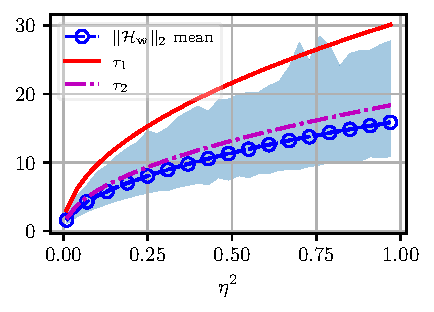
\includegraphics[width = \linewidth]{Figuras/taus_N_64_beta_0.9.pdf}
			\caption{$n = 64$}
		\end{subfigure}
		\begin{subfigure}{0.4\linewidth}
			\centering
			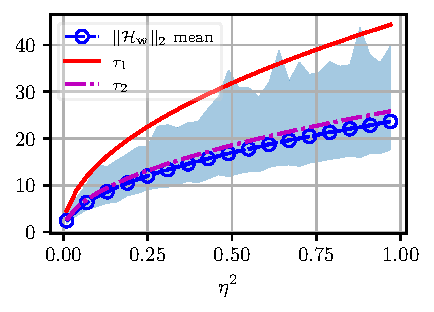
\includegraphics[width = \linewidth]{Figuras/taus_N_128_beta_0.9.pdf}
			\caption{$n = 128$}
		\end{subfigure}
		\begin{subfigure}{0.4\linewidth}
			\centering
			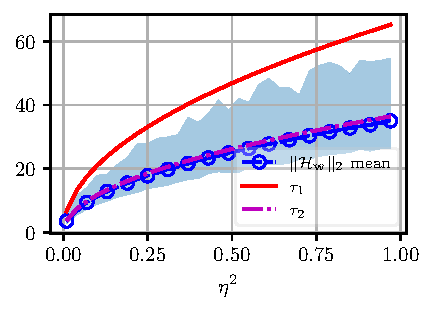
\includegraphics[width = \linewidth]{Figuras/taus_N_256_beta_0.9.pdf}
			\caption{$n = 256$}
		\end{subfigure}
		\begin{subfigure}{0.4\linewidth}
			\centering
			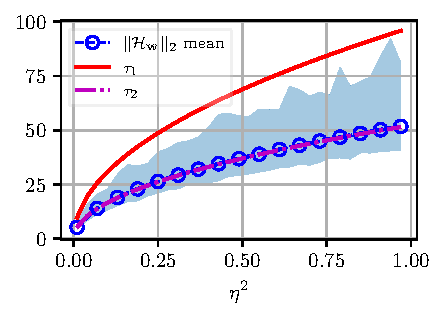
\includegraphics[width = \linewidth]{Figuras/taus_N_512_beta_0.9.pdf}
			\caption{$n = 512$}
		\end{subfigure}
		\caption{Realizaciones de $\|\Hank_\w\|_2$ y cotas $\tau_1$ y $\tau_2$ para diferentes dimensiones $n$ con $\beta = 0.9$}
		\label{fig:taus11}
	\end{figure}

\newpage




	Due to \cite{tropp2015} we have the following concentration inequality for the spectral norm of a square real random Hankel matrix.

\begin{theorem}\label{Th:boundHankelMatrix}
	Let $\H_{\w}$ be a $n\times n$ random Hankel matrix with generating vector $\w = [w_0, w_1,\cdots,w_{2n-2}]^T\sim\mathcal{N}(\mathbf{0},\eta^2\matI_n)$. Then, we have that
	\begin{equation}
		\P[\|\H_{\w}\|_2\geq t] \leq 2n \exp\bigg[-\frac{t^2}{2\eta^2n}\bigg]
		\label{Eq:BoundHankelMatrix}
	\end{equation}
\end{theorem}				
\begin{proof}
	See Appendix \ref{Proof:BoundHankelMatrix}.
\end{proof}

The result in Theorem~\ref{Th:boundHankelMatrix} is also obtained in \cite{Qiao2020} for the case of real square Toeplitz matrix. However, the bound present some difficulties. It is assumed that the entries of the Hankel matrix are real normal random variables and the expression \eqref{Eq:HankExpression} is only valid for square matrices. When we have rectangular matrix with complex random variables we can not use the results in theorem~\ref{Th:boundHankelMatrix}. In this case, we propose the following bound for the spectral norm of a Hankel matrix,

\section{Proof of theorem \ref{Th:boundHankelMatrix}} \label{Proof:BoundHankelMatrix}

In order to prove theorem \ref{Th:boundHankelMatrix}, we state the following result

\begin{lemma}\cite[Chap. 4]{tropp2015}\label{lemma:RandomMatrixIneq}
	
	Consider a finite sequence $\{\matA_k\}$ of $m\times n$ fixed complex matrices and let $\{\gamma_k\}$ be a finite sequence of independent standard normal random variables, we define a random series with matrix coefficients as									
	\begin{equation}
		\matY = \sum_k\gamma_k\matA_k.
		\label{Eq:GaussSeries}
	\end{equation}
	
	Let $\nu(\matY)$ be the matrix variance statistics of the sum
	\begin{equation}
		\begin{aligned} 
			\nu(\matY) & = \max\{\|\E[\matY\matY^H]\|_2,\|\E[\matY^H\matY]\|_2\}\\[0.3em]
			& = \max\{\|\sum_k\mathbf{A}_k\mathbf{A}_k^H\|_2,\|\sum_k\mathbf{A}_k^H\mathbf{A}_k\|_2\},
		\end{aligned}
	\end{equation}
	then, for all $t\geq 0$,
	\begin{equation}
		\P[\|\matY\|_2\geq t]\leq (m+n)\exp\bigg[-\frac{t^2}{2\nu(\matY)}\bigg]
		\label{Eq:boundGaussSeries}
	\end{equation}						
\end{lemma}

Now we demonstrate Theorem \ref{Th:boundHankelMatrix}. Consider a random vector $\w = [w_0, w_1,\cdots,w_{2n-2}]^T\sim\mathcal{N}(\mathbf{0},\eta^2\matI_n)$, the Hankel matrix can be written as																
\begin{equation}
	\H_{\w} = w_{n-1}\matJ + \sum_{k=1}^{n-1}
	w_{n-k-1}\matB^k\matJ + \sum_{k=1}^{n-1}w_{n+k-1}(\matB^k)^H\matJ,
	\label{Eq:HankExpression}
\end{equation}
where we have that
\[\matB = \begin{bmatrix} 0 & 1 & 		  &        &  \\
	& 0 & 1      &        &  \\
	&   & \ddots & \ddots &   \\
	&   &        &  0     & 1 \\
	&   &        &        & 0
\end{bmatrix}, \qquad \matJ = \begin{bmatrix} 0  & 0 & \cdots & 0 & 1\\
	0  & 0 & \cdots & 1 & 0\\
	\vdots &   & \ddots &   & \vdots \\
	1      & 0 &        & 0 & 0
\end{bmatrix}.\]

It follows that $\matJ\matJ^H = \matJ^H\matJ = \matI$ and that
\[\matB^k(\matB^k)^H = \sum_{i=1}^{n-k}\matE_{ii},\quad (\matB^k)^H\matB^k = \sum_{i=k+1}^{n}\matE_{ii},\]
where $\matE_{ii}$ is a matrix with entries equal 1 in position $ii$ and zeros otherwise.

From expression \eqref{Eq:HankExpression}, we obtain the matrix variance statistics. First, we calculate the sum of the squares of the coefficient matrices as 

\[\begin{aligned}
	\matI + \sum_{k=1}^{n-1}\matB^k(\matB^k)^H + \sum_{k=1}^{n-1}(\matB^k)^H\matB^k & = \matI + \sum_{k=1}^{n-1}\bigg[\sum_{i=1}^{n-k}\matE_{ii} + \sum_{i=k+1}^{n}\matE_{ii}\bigg]\\[0.3em]
	& = \sum_{i=1}^n\bigg[1 + \sum_{k=1}^{n-i}1+\sum_{k=1}^{i-1}1\bigg]\matE_{ii} \\
	& = \sum_{i=1}^n(1+(n-i)+(i-1))\matE_{ii} = n\matI.
\end{aligned}\]	
Then, taking expectation, we obtain
\[\nu(\H_{\w}) = \|\eta^2n\matI\|_2 = \eta^2n.\]

Finally, by lemma~\ref{lemma:RandomMatrixIneq}, we obtain the bound \eqref{Eq:BoundHankelMatrix} and the proof of Theorem.~\ref{Th:boundHankelMatrix} is completed.

	When the circulant matrix has complex Gaussian random entries, we characterize the spectral norm of the circulant random matrix with the following distribution function 

\begin{lemma}\label{Lemma:2}
	Let $N = m+n-1$, an define $R = \max_{0\leq k\leq N-1} |\mathbf{e}_{k+1}^T\matV\w|$.Then, 
	\begin{enumerate}
		\item if $\w\sim\mathcal{CN}(\mathbf{0},\eta^2\matI_{N})$, the distribution function of random variable $R$ is
		\begin{equation}
			F_R(r) = \P[R\leq r] = \bigg[1-e^{-\frac{r^2}{N\eta^2}}\bigg]^{N} \cdot\one\big\{r\geq 0\big\}
			\label{Eq:BoundCirculantMatrix2}
		\end{equation}		
		
		\item  if $\w\sim\mathcal{N}(\mathbf{0},\eta^2\matI_{N})$, the distribution function of random variable $R$ is
		\begin{equation}
			F_R(r) = \P(R\le r) = \begin{cases}\mathrm{erf}^2\bigg(\frac{r}{\eta\sqrt{2N}}\bigg)\bigg[1-e^{-\frac{r^2}{\eta^2 N}}\bigg]^{\frac{N}{2}-1} & \text{$N$ even}\\[0.3em]
				\mathrm{erf}\bigg(\frac{r}{\eta\sqrt{2N)}}\bigg)\bigg[1-e^{-\frac{r^2}{\eta^2N}}\bigg]^{\frac{N-1}{2}} & \text{$N$ odd.}
			\end{cases}
			\label{Eq:DistributionRealVector}
		\end{equation}
		for $r\ge 0$ and $\mathrm{erf}(\cdot)$ is the error function, $\mathrm{erf}(x) = \frac{2}{\sqrt{\pi}}\int_0^xe^{-t^2}\mathrm{d}t $
	\end{enumerate}						     
\end{lemma}
\begin{proof}
	See Appendix \ref{Proof:Lemma2}
\end{proof}

 When we have a random normal complex vector combining lemmas \ref{Lemma:1} and \ref{Lemma:2} we can find a new probabilistic upper bound for the spectral norm of a random Hankel matrix.

\begin{theorem}\label{Th:boundHankelMatrix2}
	Let $\H_{\w}$ be a $m\times n$ random Hankel matrix with generating vector $\w = [w_0, w_1,\cdots,w_{m+n-2}]^T\sim\mathcal{CN}(\mathbf{0},\eta^2\matI_{m+n-1})$. Then, we have that
	\begin{equation}
		\|\H_{\w}\|_2 \leq \sqrt{-(m+n-1)\eta^2\log(1-\beta^{\frac{1}{m+n-1}})} \quad \text{with prob. $\beta$,}
		\label{Eq:BoundHankelMatrix2}
	\end{equation}
	where $\beta\in(0,1)$ is such that $\P[\|\H_{\w}\|_2\le t]\ge\beta$.
\end{theorem}				

\begin{proof}
	From lemma~\ref{Lemma:2} we obtain that with probability $\beta$ that
	\[\|\matC_{\w}\|_2\le \sqrt{-(m+n-1)\eta^2\log(1-\beta^{\frac{1}{m+n-1}})}.\]
	Then, by lemma~\ref{Lemma:1} we obtain \eqref{Eq:BoundHankelMatrix2}.
\end{proof}

Unfortunately, a close expression for an upper bound for the spectral norm of real random Hankel matrix is not possible due to the complex expression of its distribution function in \eqref{Eq:DistributionRealVector}. 

In case of square $n\times n$ real random Hankel matrix we have the following concentration inequality  \cite[chap. 4]{tropp2015}


	\subsection{Proof of lemma \ref{Lemma:2}}\label{Proof:Lemma2}

\begin{enumerate} 
	\item As $\w$ is a complex random vector and $\matV$ is an unitary matrix, we have that $[\matV\w]_i\sim \mathcal{CN}(0,N\eta^2)$. If we call $Z_i = |[\matV\w]_i|$, we know that all $Z_i$s have a Rayleigh distribution with parameter $\eta\sqrt{\frac{N}{2}}$ and are independent. So the distribution of the maximum is
	
	\[F_R(r) = \P(R\le r) = \prod_{i=1}^{N}\P(Z_i\le r) = \bigg[1 - e^{-\frac{r^2}{N\eta^2}}\bigg]^{N}\cdot\one\{r\ge0\}.\]
	
	\item When $\w$ is real vector, its DFT will be even symmetric, i.e. $[\matV\w]_i=[\matV\w]^*_{-i\mod N}$ $\forall i\in\{0,\ldots,N-1\}$. Also, for even $N$ $[\matV\w]_0$ and $[\matV\w]_{N/2}$ are real value, and the DFT will be completely specified by the remainder $N/2-1$ terms. On the other hand, with an odd $N$ we have that $[\matV\w]_0$ is real and the DFT will be fully specified with the remaining $(N-1)/2$ terms. Then, it follows that
	
	\[[\matV\w]_i \sim \begin{cases} \mathcal{N}(0,N\eta^2) & \text{if $i=0$ or $i = N/2$}\\
		\mathcal{CN}(0,N\eta^2) & \text{otherwise.}
	\end{cases}\] 
	
	For $Z_i = |[\matV\w]_i|$, we have that its distribution will be
	
	\[\P[Z_i\leq z] = \begin{cases} \mathrm{erf}\bigg(\frac{z}{\eta\sqrt{2N}}\bigg) & \text{if $i=0$ or $i = N/2$}\\[0.3em] \big[1-e^{-\frac{z^2}{\eta^2N}}\big]\cdot\one\{z\ge 0\} &  \text{otherwise.}
	\end{cases} \]
	Finally, we get
	
	\[F_r(r) = \P(R\le r) = \begin{cases}\mathrm{erf}^2\bigg[\frac{r}{\eta\sqrt{2N}}\bigg]\cdot\bigg[1-e^{-\frac{r^2}{\eta^2N}}\bigg]^{\frac{N}{2}-1} & \text{$N$ even}\\
		\mathrm{erf}\bigg[\frac{r}{\eta\sqrt{2N}}\bigg]\cdot\bigg[1-e^{-\frac{r^2}{\eta^2N}}\bigg]^{\frac{N-1}{2}} & \text{$N$ odd.}
	\end{cases}\]
	
\end{enumerate}





%\section*{Apéndice}
%\addcontentsline{toc}{section}{\bfseries Apéndices}
%\renewcommand{\thesubsection}{\arabic{subsection}}
%\setcounter{subsection}{0}

